\documentclass{article}
\PassOptionsToPackage{numbers,sort&compress}{natbib}
\usepackage[preprint]{neurips_2026}
\usepackage[utf8]{inputenc}
\usepackage[T1]{fontenc}
\usepackage{amsmath,amssymb,booktabs,graphicx,microtype,xcolor,array}
\usepackage[hidelinks]{hyperref}
\usepackage{url}
\usepackage{listings}
\input{glyphtounicode}
\pdfgentounicode=1
\lstset{basicstyle=\ttfamily\scriptsize,breaklines=true,columns=fullflexible,keepspaces=true,
  breakatwhitespace=false,showstringspaces=false}
% Generated by scripts/make_numbers.py. Do not edit by hand.
\newcommand{\NBenchAll}{281}
\newcommand{\NBenchBinary}{173}
\newcommand{\NBenchNotFetched}{4}
\newcommand{\NBenchInStats}{169}
\newcommand{\NBenchNoBinary}{3}
\newcommand{\NBenchKept}{166}
\newcommand{\NItems}{329,666}
\newcommand{\NPairs}{8,810,555}
\newcommand{\NTrials}{40,775,314}
\newcommand{\NSubjectConfigs}{14,453}
\newcommand{\NSubjectsWithPairs}{11,420}
\newcommand{\NGroupsEighty}{8,765}
\newcommand{\NBenchGroupsEighty}{150}
\newcommand{\NBenchCapped}{58}
\newcommand{\PctName}{45}
\newcommand{\PctRelease}{31}
\newcommand{\PctEffort}{0.2}
\newcommand{\SkippedFetch}{mind2web, naturalreasoning, swe\_smith, tensortrust}
\newcommand{\SkippedNoBinary}{chartmuseum, ineqmath, mmmu\_dev\_val}
\newcommand{\LoboA}{0.21260}
\newcommand{\LoboARel}{$+$0.08}
\newcommand{\LoboARelAbs}{0.08}
\newcommand{\LoboB}{0.21217}
\newcommand{\LoboBRel}{$-$0.13}
\newcommand{\LoboBRelAbs}{0.13}
\newcommand{\LoboBeta}{0.21244}
\newcommand{\LoboFolds}{5}
\newcommand{\LoboGroups}{8,765}
\newcommand{\LoboBenchmarks}{150}
\newcommand{\LoboBGammaThree}{0.21217}
\newcommand{\LoboBGammaFourFive}{0.21258}
\newcommand{\LoboBGammaSix}{0.21322}
\newcommand{\LoboBGammaSevenFive}{0.21406}
\newcommand{\LoboBGammaNine}{0.21503}
\newcommand{\LoboBBzero}{0.2497}
\newcommand{\LoboC}{0.21229}
\newcommand{\LoboCRel}{$-$0.07}
\newcommand{\LoboCRelAbs}{0.07}
\newcommand{\LoboInit}{0.21523}
\newcommand{\LoboInitRel}{$+$1.32}
\newcommand{\LoboInitRelAbs}{1.32}
\newcommand{\LoboInitGammaMin}{0.7}
\newcommand{\BakeEfive}{0.21684}
\newcommand{\BakeEfiveRel}{$-$0.54}
\newcommand{\BakeEfiveRelAbs}{0.54}
\newcommand{\BakeBeta}{0.21801}
\newcommand{\BakeQwen}{0.21651}
\newcommand{\BakeQwenRel}{$-$0.68}
\newcommand{\BakeQwenRelAbs}{0.68}
\newcommand{\LoboKernel}{0.20888}
\newcommand{\LoboKernelBeta}{0.21017}
\newcommand{\DevBeta}{0.21375}
\newcommand{\DevLevel}{$-$0.0020}
\newcommand{\DevLevelAbs}{0.0020}
\newcommand{\DevExact}{$-$0.0031}
\newcommand{\DevExactAbs}{0.0031}
\newcommand{\DevKernel}{$-$0.0041}
\newcommand{\DevKernelAbs}{0.0041}
\newcommand{\DevPrior}{$-$0.0043}
\newcommand{\DevPriorAbs}{0.0043}
\newcommand{\DevPriorNoKernel}{$-$0.0034}
\newcommand{\DevPriorNoKernelAbs}{0.0034}
\newcommand{\DevPriorSix}{$-$0.0024}
\newcommand{\DevPriorSixAbs}{0.0024}
\newcommand{\GridN}{487}
\newcommand{\GridBest}{0.20877}
\newcommand{\GridDiff}{$-$0.00463}
\newcommand{\GridDiffAbs}{0.00463}
\newcommand{\GridSe}{0.00028}
\newcommand{\GridRel}{$-$2.2}
\newcommand{\GridRelAbs}{2.2}
\newcommand{\GridBeta}{0.21340}
\newcommand{\ConfDraws}{600}
\newcommand{\ConfSeedZero}{100,000}
\newcommand{\ConfSeedLast}{100,599}
\newcommand{\ConfGroups}{4,823}
\newcommand{\ConfBeta}{0.21260}
\newcommand{\ConfBetaTwo}{$+$0.00023}
\newcommand{\ConfBetaTwoAbs}{0.00023}
\newcommand{\ConfBetaTwoSe}{0.00019}
\newcommand{\ConfBetaTwoRel}{$+$0.11}
\newcommand{\ConfBetaTwoRelAbs}{0.11}
\newcommand{\ConfBetaTwoAlc}{0.21283}
\newcommand{\ConfLevel}{$-$0.00171}
\newcommand{\ConfLevelAbs}{0.00171}
\newcommand{\ConfLevelSe}{0.00016}
\newcommand{\ConfLevelRel}{$-$0.80}
\newcommand{\ConfLevelRelAbs}{0.80}
\newcommand{\ConfLevelAlc}{0.21089}
\newcommand{\ConfExact}{$-$0.00263}
\newcommand{\ConfExactAbs}{0.00263}
\newcommand{\ConfExactSe}{0.00018}
\newcommand{\ConfExactRel}{$-$1.24}
\newcommand{\ConfExactRelAbs}{1.24}
\newcommand{\ConfExactAlc}{0.20997}
\newcommand{\ConfKernel}{$-$0.00369}
\newcommand{\ConfKernelAbs}{0.00369}
\newcommand{\ConfKernelSe}{0.00022}
\newcommand{\ConfKernelRel}{$-$1.73}
\newcommand{\ConfKernelRelAbs}{1.73}
\newcommand{\ConfKernelAlc}{0.20891}
\newcommand{\ConfFull}{$-$0.00388}
\newcommand{\ConfFullAbs}{0.00388}
\newcommand{\ConfFullSe}{0.00023}
\newcommand{\ConfFullRel}{$-$1.82}
\newcommand{\ConfFullRelAbs}{1.82}
\newcommand{\ConfFullAlc}{0.20872}
\newcommand{\ConfPriorOnly}{$-$0.00195}
\newcommand{\ConfPriorOnlyAbs}{0.00195}
\newcommand{\ConfPriorOnlySe}{0.00019}
\newcommand{\ConfPriorOnlyRel}{$-$0.92}
\newcommand{\ConfPriorOnlyRelAbs}{0.92}
\newcommand{\ConfPriorOnlyAlc}{0.21065}
\newcommand{\ConfGammaOne}{$+$0.00002}
\newcommand{\ConfGammaOneAbs}{0.00002}
\newcommand{\ConfGammaOneSe}{0.00037}
\newcommand{\ConfGammaOneRel}{$+$0.01}
\newcommand{\ConfGammaOneRelAbs}{0.01}
\newcommand{\ConfGammaOneAlc}{0.21262}
\newcommand{\ConfFullBzero}{0.2492}
\newcommand{\ConfFullBlast}{0.1810}
\newcommand{\ConfBetaBlast}{0.188}
\newcommand{\ConfPriorGain}{$-$0.00019}
\newcommand{\ConfPriorGainAbs}{0.00019}
\newcommand{\ConfShareStructure}{95}
\newcommand{\SimDrawSd}{0.027}
\newcommand{\SimPairSd}{0.0057}
\newcommand{\ConfNine}{119}
\newcommand{\ConfEight}{385}
\newcommand{\ConfSeven}{96}
\newcommand{\OffTables}{10}
\newcommand{\OffPairsMin}{44}
\newcommand{\OffPairsMax}{76}
\newcommand{\OffPairsLarge}{2}
\newcommand{\OffPairsLargeValue}{113}
\newcommand{\OffTablesNine}{8}
\newcommand{\OffTablesEight}{2}
\newcommand{\OffGroupEvals}{88}
\newcommand{\OffDistinctGroups}{70}
\newcommand{\OffDistinctBench}{7}
\newcommand{\OffBetaLaterN}{3}
\newcommand{\OffBetaAllSd}{0.0174}
\newcommand{\OffBetaLaterRuns}{0.2190, 0.1777, 0.1835}
\newcommand{\OffBetaLaterMean}{0.1934}
\newcommand{\TabBetaLaterRow}{Beta(2,2), runs after model selection & 3 & 0.2190, 0.1777, 0.1835 & 0.1934 (0.0129) \\}
\newcommand{\OffBetaN}{3}
\newcommand{\OffBetaMean}{0.1778}
\newcommand{\OffBetaSd}{0.0085}
\newcommand{\OffBetaSe}{0.0049}
\newcommand{\OffBetaRuns}{0.1867, 0.1698, 0.1769}
\newcommand{\OffBetaRange}{0.0169}
\newcommand{\OffVtwo}{0.1695}
\newcommand{\UnscoredAsOf}{5 November 03:04 UTC}
\newcommand{\TabVtwoRuns}{1 (2 not started)}
\newcommand{\TabVtwoAlc}{0.1695}
\newcommand{\TabVtwoMean}{}
\newcommand{\OffVtwoN}{1}
\newcommand{\TabLfiveRuns}{0 (4 not started)}
\newcommand{\TabLfiveAlc}{none}
\newcommand{\TabLfiveMean}{}
\newcommand{\OffLfiveN}{0}
\newcommand{\LfiveOfficialSentence}{Finally, the stalled platform queue left L5 without an official run by \UnscoredAsOf.}
\newcommand{\OffVtwoBzero}{0.2536}
\newcommand{\OffVthree}{0.1711}
\newcommand{\OffVthreeBzero}{0.2401}
\newcommand{\OffBetaBlastMin}{0.128}
\newcommand{\OffBetaBlastMax}{0.153}
\newcommand{\RunsNeededLow}{268}
\newcommand{\RunsNeededHigh}{602}
\newcommand{\RunsNeededOurs}{316}
\newcommand{\SpreadRatio}{13}
\newcommand{\OffBetaAllN}{6}
\newcommand{\OffBetaAllRuns}{0.1867, 0.1698, 0.1769, 0.2190, 0.1777, 0.1835}
\newcommand{\OffBetaAllMean}{0.1856}
\newcommand{\OffBetaAllSe}{0.0071}
\newcommand{\OffBetaAllRange}{0.0493}
\newcommand{\RunsNeededPaired}{18}
\newcommand{\BestOfTwentyShift}{0.030}
\newcommand{\ConfGammaOneBzero}{0.2579}
\newcommand{\ConfFullSeRel}{0.11}
\newcommand{\ConfPriorStep}{$-$0.00020}
\newcommand{\ConfPriorStepAbs}{0.00020}
\newcommand{\ConfPriorStepSe}{0.00009}
\newcommand{\ConfPriorLevel}{$-$0.00025}
\newcommand{\ConfPriorLevelAbs}{0.00025}
\newcommand{\ConfPriorLevelSe}{0.00009}
\newcommand{\EmbedSeconds}{822}
\newcommand{\ArchiveFullMB}{282.6}
\newcommand{\ArchiveLevelMB}{1.3}
\newcommand{\PriorMB}{1.4}
\newcommand{\JudgeItems}{18,952}
\newcommand{\VthreeResponses}{1,142,294}
\newcommand{\VthreeGroups}{82}
\newcommand{\TrialRatio}{36}
\newcommand{\VtwoResponses}{1,073,030}
\newcommand{\OfficialRows}{1003760 & Beta(2,2) baseline & 9 & 7 & 0.1867 & 0.2500 & 0.1496 \\
1003791 & V1 hierarchical prior & 8 & 7 & 0.1911 & 0.2511 & 0.1612 \\
1004759 & V2 & 9 & 7 & 0.1695 & 0.2536 & 0.1330 \\
1004796 & V3 & 9 & 7 & 0.1711 & 0.2401 & 0.1478 \\
1004970 & V3 with uncertainty band & 9 & 7 & 0.1876 & 0.2341 & 0.1644 \\
1032881 & Beta(2,2) baseline & 9 & 7 & 0.1698 & 0.2500 & 0.1277 \\
1032882 & Beta(2,2) baseline & 8 & 7 & 0.1769 & 0.2500 & 0.1533 \\
1034630 & Beta(2,2) baseline & 9 & 7 & 0.2190 & 0.2500 & 0.1824 \\
1034631 & Beta(2,2) baseline & 9 & 7 & 0.1777 & 0.2500 & 0.1404 \\
1034661 & Beta(2,2) baseline & 9 & 7 & 0.1835 & 0.2500 & 0.1429 \\}
\newcommand{\TpGroups}{26}
\newcommand{\TpPq}{0.136}
\newcommand{\TrainPq}{0.184}
\newcommand{\TrainP}{0.510}
\newcommand{\TrainAbove}{55}
\newcommand{\RecentP}{0.614}
\newcommand{\RecentAbove}{68}
\newcommand{\RecentGroups}{328}
\newcommand{\RecentBench}{35}
\newcommand{\TpShareOwn}{0.115, 0.077, 0.231, 0.308, 0.269}
\newcommand{\TpLaterGroups}{27}
\newcommand{\TpLaterShare}{0.185, 0.222, 0.148, 0.148, 0.296}
\newcommand{\TpLaterPq}{0.151}
\newcommand{\TpPooledGroups}{53}
\newcommand{\TpShareSim}{0.115, 0.077, 0.192, 0.308, 0.308}
\newcommand{\TpFarShare}{58}
\newcommand{\TpExtremeN}{7}
\newcommand{\DateA}{-0.472}
\newcommand{\DateB}{0.285}
\newcommand{\DateAzero}{-0.093}
\newcommand{\LadRDDraws}{600}
\newcommand{\LadRDGroups}{4,832}
\newcommand{\LadRDBench}{56}
\newcommand{\LadRDUBeta}{0.2113}
\newcommand{\LadRDULonec}{$-$0.0033}
\newcommand{\LadRDULonecAbs}{0.0033}
\newcommand{\LadRDULonecSe}{0.0002}
\newcommand{\LadRDULtwoc}{$-$0.0061}
\newcommand{\LadRDULtwocAbs}{0.0061}
\newcommand{\LadRDULtwocSe}{0.0002}
\newcommand{\LadRDUWlevel}{$-$0.0006}
\newcommand{\LadRDUWlevelAbs}{0.0006}
\newcommand{\LadRDUWlevelSe}{0.0002}
\newcommand{\LadRDUWexact}{$-$0.0014}
\newcommand{\LadRDUWexactAbs}{0.0014}
\newcommand{\LadRDUWexactSe}{0.0002}
\newcommand{\LadRDUWkernel}{$-$0.0028}
\newcommand{\LadRDUWkernelAbs}{0.0028}
\newcommand{\LadRDUWkernelSe}{0.0002}
\newcommand{\LadRDULthree}{$-$0.0035}
\newcommand{\LadRDULthreeAbs}{0.0035}
\newcommand{\LadRDULthreeSe}{0.0002}
\newcommand{\LadRDULfour}{$-$0.0039}
\newcommand{\LadRDULfourAbs}{0.0039}
\newcommand{\LadRDULfourSe}{0.0002}
\newcommand{\LadRDULfive}{$-$0.0042}
\newcommand{\LadRDULfiveAbs}{0.0042}
\newcommand{\LadRDULfiveSe}{0.0002}
\newcommand{\LadRDULfivent}{$-$0.0037}
\newcommand{\LadRDULfiventAbs}{0.0037}
\newcommand{\LadRDULfiventSe}{0.0002}
\newcommand{\LadRDULsix}{$-$0.0051}
\newcommand{\LadRDULsixAbs}{0.0051}
\newcommand{\LadRDULsixSe}{0.0003}
\newcommand{\LadRDULfiveRel}{$-$2.0}
\newcommand{\LadRDULfiveRelAbs}{2.0}
\newcommand{\LadRDTBeta}{0.1747}
\newcommand{\LadRDTLonec}{$+$0.0001}
\newcommand{\LadRDTLonecAbs}{0.0001}
\newcommand{\LadRDTLonecSe}{0.0002}
\newcommand{\LadRDTLtwoc}{$-$0.0045}
\newcommand{\LadRDTLtwocAbs}{0.0045}
\newcommand{\LadRDTLtwocSe}{0.0003}
\newcommand{\LadRDTWlevel}{$-$0.0032}
\newcommand{\LadRDTWlevelAbs}{0.0032}
\newcommand{\LadRDTWlevelSe}{0.0002}
\newcommand{\LadRDTWexact}{$-$0.0037}
\newcommand{\LadRDTWexactAbs}{0.0037}
\newcommand{\LadRDTWexactSe}{0.0002}
\newcommand{\LadRDTWkernel}{$-$0.0048}
\newcommand{\LadRDTWkernelAbs}{0.0048}
\newcommand{\LadRDTWkernelSe}{0.0002}
\newcommand{\LadRDTLthree}{$-$0.0060}
\newcommand{\LadRDTLthreeAbs}{0.0060}
\newcommand{\LadRDTLthreeSe}{0.0002}
\newcommand{\LadRDTLfour}{$-$0.0067}
\newcommand{\LadRDTLfourAbs}{0.0067}
\newcommand{\LadRDTLfourSe}{0.0002}
\newcommand{\LadRDTLfive}{$-$0.0074}
\newcommand{\LadRDTLfiveAbs}{0.0074}
\newcommand{\LadRDTLfiveSe}{0.0003}
\newcommand{\LadRDTLfivent}{$-$0.0066}
\newcommand{\LadRDTLfiventAbs}{0.0066}
\newcommand{\LadRDTLfiventSe}{0.0002}
\newcommand{\LadRDTLsix}{$-$0.0079}
\newcommand{\LadRDTLsixAbs}{0.0079}
\newcommand{\LadRDTLsixSe}{0.0003}
\newcommand{\LadRDTLfiveRel}{$-$4.2}
\newcommand{\LadRDTLfiveRelAbs}{4.2}
\newcommand{\LadRDOBeta}{0.1792}
\newcommand{\LadRDOLonec}{$-$0.0004}
\newcommand{\LadRDOLonecAbs}{0.0004}
\newcommand{\LadRDOLonecSe}{0.0002}
\newcommand{\LadRDOLtwoc}{$-$0.0047}
\newcommand{\LadRDOLtwocAbs}{0.0047}
\newcommand{\LadRDOLtwocSe}{0.0002}
\newcommand{\LadRDOWlevel}{$-$0.0029}
\newcommand{\LadRDOWlevelAbs}{0.0029}
\newcommand{\LadRDOWlevelSe}{0.0002}
\newcommand{\LadRDOWexact}{$-$0.0034}
\newcommand{\LadRDOWexactAbs}{0.0034}
\newcommand{\LadRDOWexactSe}{0.0002}
\newcommand{\LadRDOWkernel}{$-$0.0046}
\newcommand{\LadRDOWkernelAbs}{0.0046}
\newcommand{\LadRDOWkernelSe}{0.0002}
\newcommand{\LadRDOLthree}{$-$0.0057}
\newcommand{\LadRDOLthreeAbs}{0.0057}
\newcommand{\LadRDOLthreeSe}{0.0002}
\newcommand{\LadRDOLfour}{$-$0.0064}
\newcommand{\LadRDOLfourAbs}{0.0064}
\newcommand{\LadRDOLfourSe}{0.0002}
\newcommand{\LadRDOLfive}{$-$0.0070}
\newcommand{\LadRDOLfiveAbs}{0.0070}
\newcommand{\LadRDOLfiveSe}{0.0003}
\newcommand{\LadRDOLfivent}{$-$0.0062}
\newcommand{\LadRDOLfiventAbs}{0.0062}
\newcommand{\LadRDOLfiventSe}{0.0002}
\newcommand{\LadRDOLsix}{$-$0.0075}
\newcommand{\LadRDOLsixAbs}{0.0075}
\newcommand{\LadRDOLsixSe}{0.0003}
\newcommand{\LadRDOLfiveRel}{$-$3.9}
\newcommand{\LadRDOLfiveRelAbs}{3.9}
\newcommand{\LadRFDraws}{600}
\newcommand{\LadRFGroups}{4,807}
\newcommand{\LadRFBench}{56}
\newcommand{\LadRFUBeta}{0.2110}
\newcommand{\LadRFULonec}{$-$0.0033}
\newcommand{\LadRFULonecAbs}{0.0033}
\newcommand{\LadRFULonecSe}{0.0002}
\newcommand{\LadRFULtwoc}{$-$0.0060}
\newcommand{\LadRFULtwocAbs}{0.0060}
\newcommand{\LadRFULtwocSe}{0.0002}
\newcommand{\LadRFUWlevel}{$-$0.0008}
\newcommand{\LadRFUWlevelAbs}{0.0008}
\newcommand{\LadRFUWlevelSe}{0.0002}
\newcommand{\LadRFUWexact}{$-$0.0015}
\newcommand{\LadRFUWexactAbs}{0.0015}
\newcommand{\LadRFUWexactSe}{0.0002}
\newcommand{\LadRFUWkernel}{$-$0.0030}
\newcommand{\LadRFUWkernelAbs}{0.0030}
\newcommand{\LadRFUWkernelSe}{0.0002}
\newcommand{\LadRFULthree}{$-$0.0037}
\newcommand{\LadRFULthreeAbs}{0.0037}
\newcommand{\LadRFULthreeSe}{0.0002}
\newcommand{\LadRFULfour}{$-$0.0041}
\newcommand{\LadRFULfourAbs}{0.0041}
\newcommand{\LadRFULfourSe}{0.0002}
\newcommand{\LadRFULfive}{$-$0.0043}
\newcommand{\LadRFULfiveAbs}{0.0043}
\newcommand{\LadRFULfiveSe}{0.0002}
\newcommand{\LadRFULfivent}{$-$0.0038}
\newcommand{\LadRFULfiventAbs}{0.0038}
\newcommand{\LadRFULfiventSe}{0.0002}
\newcommand{\LadRFULsix}{$-$0.0051}
\newcommand{\LadRFULsixAbs}{0.0051}
\newcommand{\LadRFULsixSe}{0.0003}
\newcommand{\LadRFULfiveRel}{$-$2.0}
\newcommand{\LadRFULfiveRelAbs}{2.0}
\newcommand{\LadRFTBeta}{0.1746}
\newcommand{\LadRFTLonec}{$+$0.0000}
\newcommand{\LadRFTLonecAbs}{0.0000}
\newcommand{\LadRFTLonecSe}{0.0002}
\newcommand{\LadRFTLtwoc}{$-$0.0047}
\newcommand{\LadRFTLtwocAbs}{0.0047}
\newcommand{\LadRFTLtwocSe}{0.0002}
\newcommand{\LadRFTWlevel}{$-$0.0035}
\newcommand{\LadRFTWlevelAbs}{0.0035}
\newcommand{\LadRFTWlevelSe}{0.0002}
\newcommand{\LadRFTWexact}{$-$0.0040}
\newcommand{\LadRFTWexactAbs}{0.0040}
\newcommand{\LadRFTWexactSe}{0.0002}
\newcommand{\LadRFTWkernel}{$-$0.0052}
\newcommand{\LadRFTWkernelAbs}{0.0052}
\newcommand{\LadRFTWkernelSe}{0.0002}
\newcommand{\LadRFTLthree}{$-$0.0064}
\newcommand{\LadRFTLthreeAbs}{0.0064}
\newcommand{\LadRFTLthreeSe}{0.0002}
\newcommand{\LadRFTLfour}{$-$0.0071}
\newcommand{\LadRFTLfourAbs}{0.0071}
\newcommand{\LadRFTLfourSe}{0.0002}
\newcommand{\LadRFTLfive}{$-$0.0077}
\newcommand{\LadRFTLfiveAbs}{0.0077}
\newcommand{\LadRFTLfiveSe}{0.0003}
\newcommand{\LadRFTLfivent}{$-$0.0069}
\newcommand{\LadRFTLfiventAbs}{0.0069}
\newcommand{\LadRFTLfiventSe}{0.0002}
\newcommand{\LadRFTLsix}{$-$0.0082}
\newcommand{\LadRFTLsixAbs}{0.0082}
\newcommand{\LadRFTLsixSe}{0.0003}
\newcommand{\LadRFTLfiveRel}{$-$4.4}
\newcommand{\LadRFTLfiveRelAbs}{4.4}
\newcommand{\LadRFOBeta}{0.1791}
\newcommand{\LadRFOLonec}{$-$0.0004}
\newcommand{\LadRFOLonecAbs}{0.0004}
\newcommand{\LadRFOLonecSe}{0.0002}
\newcommand{\LadRFOLtwoc}{$-$0.0049}
\newcommand{\LadRFOLtwocAbs}{0.0049}
\newcommand{\LadRFOLtwocSe}{0.0002}
\newcommand{\LadRFOWlevel}{$-$0.0032}
\newcommand{\LadRFOWlevelAbs}{0.0032}
\newcommand{\LadRFOWlevelSe}{0.0002}
\newcommand{\LadRFOWexact}{$-$0.0037}
\newcommand{\LadRFOWexactAbs}{0.0037}
\newcommand{\LadRFOWexactSe}{0.0002}
\newcommand{\LadRFOWkernel}{$-$0.0050}
\newcommand{\LadRFOWkernelAbs}{0.0050}
\newcommand{\LadRFOWkernelSe}{0.0002}
\newcommand{\LadRFOLthree}{$-$0.0061}
\newcommand{\LadRFOLthreeAbs}{0.0061}
\newcommand{\LadRFOLthreeSe}{0.0002}
\newcommand{\LadRFOLfour}{$-$0.0068}
\newcommand{\LadRFOLfourAbs}{0.0068}
\newcommand{\LadRFOLfourSe}{0.0002}
\newcommand{\LadRFOLfive}{$-$0.0073}
\newcommand{\LadRFOLfiveAbs}{0.0073}
\newcommand{\LadRFOLfiveSe}{0.0003}
\newcommand{\LadRFOLfivent}{$-$0.0065}
\newcommand{\LadRFOLfiventAbs}{0.0065}
\newcommand{\LadRFOLfiventSe}{0.0002}
\newcommand{\LadRFOLsix}{$-$0.0077}
\newcommand{\LadRFOLsixAbs}{0.0077}
\newcommand{\LadRFOLsixSe}{0.0003}
\newcommand{\LadRFOLfiveRel}{$-$4.1}
\newcommand{\LadRFOLfiveRelAbs}{4.1}
\newcommand{\LadADDraws}{600}
\newcommand{\LadADGroups}{4,779}
\newcommand{\LadADBench}{150}
\newcommand{\LadADUBeta}{0.2138}
\newcommand{\LadADULonec}{$-$0.0030}
\newcommand{\LadADULonecAbs}{0.0030}
\newcommand{\LadADULonecSe}{0.0002}
\newcommand{\LadADULtwoc}{$-$0.0045}
\newcommand{\LadADULtwocAbs}{0.0045}
\newcommand{\LadADULtwocSe}{0.0002}
\newcommand{\LadADUWlevel}{$-$0.0002}
\newcommand{\LadADUWlevelAbs}{0.0002}
\newcommand{\LadADUWlevelSe}{0.0002}
\newcommand{\LadADUWexact}{$-$0.0009}
\newcommand{\LadADUWexactAbs}{0.0009}
\newcommand{\LadADUWexactSe}{0.0002}
\newcommand{\LadADUWkernel}{$-$0.0022}
\newcommand{\LadADUWkernelAbs}{0.0022}
\newcommand{\LadADUWkernelSe}{0.0002}
\newcommand{\LadADULthree}{$-$0.0024}
\newcommand{\LadADULthreeAbs}{0.0024}
\newcommand{\LadADULthreeSe}{0.0002}
\newcommand{\LadADULfour}{$-$0.0025}
\newcommand{\LadADULfourAbs}{0.0025}
\newcommand{\LadADULfourSe}{0.0002}
\newcommand{\LadADULfive}{$-$0.0024}
\newcommand{\LadADULfiveAbs}{0.0024}
\newcommand{\LadADULfiveSe}{0.0002}
\newcommand{\LadADULfivent}{$-$0.0024}
\newcommand{\LadADULfiventAbs}{0.0024}
\newcommand{\LadADULfiventSe}{0.0002}
\newcommand{\LadADULsix}{$-$0.0025}
\newcommand{\LadADULsixAbs}{0.0025}
\newcommand{\LadADULsixSe}{0.0003}
\newcommand{\LadADULfiveRel}{$-$1.1}
\newcommand{\LadADULfiveRelAbs}{1.1}
\newcommand{\LadADTBeta}{0.1716}
\newcommand{\LadADTLonec}{$+$0.0006}
\newcommand{\LadADTLonecAbs}{0.0006}
\newcommand{\LadADTLonecSe}{0.0002}
\newcommand{\LadADTLtwoc}{$-$0.0025}
\newcommand{\LadADTLtwocAbs}{0.0025}
\newcommand{\LadADTLtwocSe}{0.0003}
\newcommand{\LadADTWlevel}{$-$0.0033}
\newcommand{\LadADTWlevelAbs}{0.0033}
\newcommand{\LadADTWlevelSe}{0.0002}
\newcommand{\LadADTWexact}{$-$0.0038}
\newcommand{\LadADTWexactAbs}{0.0038}
\newcommand{\LadADTWexactSe}{0.0002}
\newcommand{\LadADTWkernel}{$-$0.0051}
\newcommand{\LadADTWkernelAbs}{0.0051}
\newcommand{\LadADTWkernelSe}{0.0002}
\newcommand{\LadADTLthree}{$-$0.0054}
\newcommand{\LadADTLthreeAbs}{0.0054}
\newcommand{\LadADTLthreeSe}{0.0003}
\newcommand{\LadADTLfour}{$-$0.0057}
\newcommand{\LadADTLfourAbs}{0.0057}
\newcommand{\LadADTLfourSe}{0.0003}
\newcommand{\LadADTLfive}{$-$0.0058}
\newcommand{\LadADTLfiveAbs}{0.0058}
\newcommand{\LadADTLfiveSe}{0.0003}
\newcommand{\LadADTLfivent}{$-$0.0056}
\newcommand{\LadADTLfiventAbs}{0.0056}
\newcommand{\LadADTLfiventSe}{0.0003}
\newcommand{\LadADTLsix}{$-$0.0050}
\newcommand{\LadADTLsixAbs}{0.0050}
\newcommand{\LadADTLsixSe}{0.0003}
\newcommand{\LadADTLfiveRel}{$-$3.4}
\newcommand{\LadADTLfiveRelAbs}{3.4}
\newcommand{\LadADOBeta}{0.1766}
\newcommand{\LadADOLonec}{$+$0.0002}
\newcommand{\LadADOLonecAbs}{0.0002}
\newcommand{\LadADOLonecSe}{0.0002}
\newcommand{\LadADOLtwoc}{$-$0.0027}
\newcommand{\LadADOLtwocAbs}{0.0027}
\newcommand{\LadADOLtwocSe}{0.0003}
\newcommand{\LadADOWlevel}{$-$0.0030}
\newcommand{\LadADOWlevelAbs}{0.0030}
\newcommand{\LadADOWlevelSe}{0.0002}
\newcommand{\LadADOWexact}{$-$0.0035}
\newcommand{\LadADOWexactAbs}{0.0035}
\newcommand{\LadADOWexactSe}{0.0002}
\newcommand{\LadADOWkernel}{$-$0.0048}
\newcommand{\LadADOWkernelAbs}{0.0048}
\newcommand{\LadADOWkernelSe}{0.0002}
\newcommand{\LadADOLthree}{$-$0.0051}
\newcommand{\LadADOLthreeAbs}{0.0051}
\newcommand{\LadADOLthreeSe}{0.0002}
\newcommand{\LadADOLfour}{$-$0.0053}
\newcommand{\LadADOLfourAbs}{0.0053}
\newcommand{\LadADOLfourSe}{0.0003}
\newcommand{\LadADOLfive}{$-$0.0053}
\newcommand{\LadADOLfiveAbs}{0.0053}
\newcommand{\LadADOLfiveSe}{0.0003}
\newcommand{\LadADOLfivent}{$-$0.0052}
\newcommand{\LadADOLfiventAbs}{0.0052}
\newcommand{\LadADOLfiventSe}{0.0003}
\newcommand{\LadADOLsix}{$-$0.0047}
\newcommand{\LadADOLsixAbs}{0.0047}
\newcommand{\LadADOLsixSe}{0.0003}
\newcommand{\LadADOLfiveRel}{$-$3.0}
\newcommand{\LadADOLfiveRelAbs}{3.0}
\newcommand{\LadAFDraws}{600}
\newcommand{\LadAFGroups}{4,791}
\newcommand{\LadAFBench}{150}
\newcommand{\LadAFUBeta}{0.2119}
\newcommand{\LadAFULonec}{$-$0.0027}
\newcommand{\LadAFULonecAbs}{0.0027}
\newcommand{\LadAFULonecSe}{0.0002}
\newcommand{\LadAFULtwoc}{$-$0.0041}
\newcommand{\LadAFULtwocAbs}{0.0041}
\newcommand{\LadAFULtwocSe}{0.0002}
\newcommand{\LadAFUWlevel}{$-$0.0003}
\newcommand{\LadAFUWlevelAbs}{0.0003}
\newcommand{\LadAFUWlevelSe}{0.0002}
\newcommand{\LadAFUWexact}{$-$0.0010}
\newcommand{\LadAFUWexactAbs}{0.0010}
\newcommand{\LadAFUWexactSe}{0.0002}
\newcommand{\LadAFUWkernel}{$-$0.0023}
\newcommand{\LadAFUWkernelAbs}{0.0023}
\newcommand{\LadAFUWkernelSe}{0.0002}
\newcommand{\LadAFULthree}{$-$0.0024}
\newcommand{\LadAFULthreeAbs}{0.0024}
\newcommand{\LadAFULthreeSe}{0.0002}
\newcommand{\LadAFULfour}{$-$0.0025}
\newcommand{\LadAFULfourAbs}{0.0025}
\newcommand{\LadAFULfourSe}{0.0002}
\newcommand{\LadAFULfive}{$-$0.0024}
\newcommand{\LadAFULfiveAbs}{0.0024}
\newcommand{\LadAFULfiveSe}{0.0002}
\newcommand{\LadAFULfivent}{$-$0.0024}
\newcommand{\LadAFULfiventAbs}{0.0024}
\newcommand{\LadAFULfiventSe}{0.0002}
\newcommand{\LadAFULsix}{$-$0.0025}
\newcommand{\LadAFULsixAbs}{0.0025}
\newcommand{\LadAFULsixSe}{0.0003}
\newcommand{\LadAFULfiveRel}{$-$1.1}
\newcommand{\LadAFULfiveRelAbs}{1.1}
\newcommand{\LadAFTBeta}{0.1710}
\newcommand{\LadAFTLonec}{$+$0.0009}
\newcommand{\LadAFTLonecAbs}{0.0009}
\newcommand{\LadAFTLonecSe}{0.0002}
\newcommand{\LadAFTLtwoc}{$-$0.0023}
\newcommand{\LadAFTLtwocAbs}{0.0023}
\newcommand{\LadAFTLtwocSe}{0.0003}
\newcommand{\LadAFTWlevel}{$-$0.0034}
\newcommand{\LadAFTWlevelAbs}{0.0034}
\newcommand{\LadAFTWlevelSe}{0.0002}
\newcommand{\LadAFTWexact}{$-$0.0038}
\newcommand{\LadAFTWexactAbs}{0.0038}
\newcommand{\LadAFTWexactSe}{0.0002}
\newcommand{\LadAFTWkernel}{$-$0.0051}
\newcommand{\LadAFTWkernelAbs}{0.0051}
\newcommand{\LadAFTWkernelSe}{0.0002}
\newcommand{\LadAFTLthree}{$-$0.0055}
\newcommand{\LadAFTLthreeAbs}{0.0055}
\newcommand{\LadAFTLthreeSe}{0.0003}
\newcommand{\LadAFTLfour}{$-$0.0058}
\newcommand{\LadAFTLfourAbs}{0.0058}
\newcommand{\LadAFTLfourSe}{0.0003}
\newcommand{\LadAFTLfive}{$-$0.0058}
\newcommand{\LadAFTLfiveAbs}{0.0058}
\newcommand{\LadAFTLfiveSe}{0.0003}
\newcommand{\LadAFTLfivent}{$-$0.0056}
\newcommand{\LadAFTLfiventAbs}{0.0056}
\newcommand{\LadAFTLfiventSe}{0.0003}
\newcommand{\LadAFTLsix}{$-$0.0050}
\newcommand{\LadAFTLsixAbs}{0.0050}
\newcommand{\LadAFTLsixSe}{0.0003}
\newcommand{\LadAFTLfiveRel}{$-$3.4}
\newcommand{\LadAFTLfiveRelAbs}{3.4}
\newcommand{\LadAFOBeta}{0.1759}
\newcommand{\LadAFOLonec}{$+$0.0005}
\newcommand{\LadAFOLonecAbs}{0.0005}
\newcommand{\LadAFOLonecSe}{0.0002}
\newcommand{\LadAFOLtwoc}{$-$0.0025}
\newcommand{\LadAFOLtwocAbs}{0.0025}
\newcommand{\LadAFOLtwocSe}{0.0003}
\newcommand{\LadAFOWlevel}{$-$0.0030}
\newcommand{\LadAFOWlevelAbs}{0.0030}
\newcommand{\LadAFOWlevelSe}{0.0002}
\newcommand{\LadAFOWexact}{$-$0.0035}
\newcommand{\LadAFOWexactAbs}{0.0035}
\newcommand{\LadAFOWexactSe}{0.0002}
\newcommand{\LadAFOWkernel}{$-$0.0048}
\newcommand{\LadAFOWkernelAbs}{0.0048}
\newcommand{\LadAFOWkernelSe}{0.0002}
\newcommand{\LadAFOLthree}{$-$0.0051}
\newcommand{\LadAFOLthreeAbs}{0.0051}
\newcommand{\LadAFOLthreeSe}{0.0002}
\newcommand{\LadAFOLfour}{$-$0.0054}
\newcommand{\LadAFOLfourAbs}{0.0054}
\newcommand{\LadAFOLfourSe}{0.0003}
\newcommand{\LadAFOLfive}{$-$0.0054}
\newcommand{\LadAFOLfiveAbs}{0.0054}
\newcommand{\LadAFOLfiveSe}{0.0003}
\newcommand{\LadAFOLfivent}{$-$0.0052}
\newcommand{\LadAFOLfiventAbs}{0.0052}
\newcommand{\LadAFOLfiventSe}{0.0003}
\newcommand{\LadAFOLsix}{$-$0.0046}
\newcommand{\LadAFOLsixAbs}{0.0046}
\newcommand{\LadAFOLsixSe}{0.0003}
\newcommand{\LadAFOLfiveRel}{$-$3.1}
\newcommand{\LadAFOLfiveRelAbs}{3.1}
\newcommand{\LadRCDraws}{600}
\newcommand{\LadRCGroups}{4,814}
\newcommand{\LadRCBench}{56}
\newcommand{\LadRCUBeta}{0.2099}
\newcommand{\LadRCULonec}{$-$0.0033}
\newcommand{\LadRCULonecAbs}{0.0033}
\newcommand{\LadRCULonecSe}{0.0001}
\newcommand{\LadRCULtwoc}{$-$0.0062}
\newcommand{\LadRCULtwocAbs}{0.0062}
\newcommand{\LadRCULtwocSe}{0.0002}
\newcommand{\LadRCUWlevel}{$-$0.0008}
\newcommand{\LadRCUWlevelAbs}{0.0008}
\newcommand{\LadRCUWlevelSe}{0.0002}
\newcommand{\LadRCUWexact}{$-$0.0016}
\newcommand{\LadRCUWexactAbs}{0.0016}
\newcommand{\LadRCUWexactSe}{0.0002}
\newcommand{\LadRCUWkernel}{$-$0.0032}
\newcommand{\LadRCUWkernelAbs}{0.0032}
\newcommand{\LadRCUWkernelSe}{0.0002}
\newcommand{\LadRCULthree}{$-$0.0039}
\newcommand{\LadRCULthreeAbs}{0.0039}
\newcommand{\LadRCULthreeSe}{0.0002}
\newcommand{\LadRCULfour}{$-$0.0043}
\newcommand{\LadRCULfourAbs}{0.0043}
\newcommand{\LadRCULfourSe}{0.0002}
\newcommand{\LadRCULfive}{$-$0.0044}
\newcommand{\LadRCULfiveAbs}{0.0044}
\newcommand{\LadRCULfiveSe}{0.0002}
\newcommand{\LadRCULfivent}{$-$0.0039}
\newcommand{\LadRCULfiventAbs}{0.0039}
\newcommand{\LadRCULfiventSe}{0.0002}
\newcommand{\LadRCULsix}{$-$0.0051}
\newcommand{\LadRCULsixAbs}{0.0051}
\newcommand{\LadRCULsixSe}{0.0003}
\newcommand{\LadRCULfiveRel}{$-$2.1}
\newcommand{\LadRCULfiveRelAbs}{2.1}
\newcommand{\LadRCTBeta}{0.1740}
\newcommand{\LadRCTLonec}{$+$0.0001}
\newcommand{\LadRCTLonecAbs}{0.0001}
\newcommand{\LadRCTLonecSe}{0.0002}
\newcommand{\LadRCTLtwoc}{$-$0.0046}
\newcommand{\LadRCTLtwocAbs}{0.0046}
\newcommand{\LadRCTLtwocSe}{0.0002}
\newcommand{\LadRCTWlevel}{$-$0.0035}
\newcommand{\LadRCTWlevelAbs}{0.0035}
\newcommand{\LadRCTWlevelSe}{0.0002}
\newcommand{\LadRCTWexact}{$-$0.0040}
\newcommand{\LadRCTWexactAbs}{0.0040}
\newcommand{\LadRCTWexactSe}{0.0002}
\newcommand{\LadRCTWkernel}{$-$0.0054}
\newcommand{\LadRCTWkernelAbs}{0.0054}
\newcommand{\LadRCTWkernelSe}{0.0002}
\newcommand{\LadRCTLthree}{$-$0.0065}
\newcommand{\LadRCTLthreeAbs}{0.0065}
\newcommand{\LadRCTLthreeSe}{0.0002}
\newcommand{\LadRCTLfour}{$-$0.0071}
\newcommand{\LadRCTLfourAbs}{0.0071}
\newcommand{\LadRCTLfourSe}{0.0002}
\newcommand{\LadRCTLfive}{$-$0.0076}
\newcommand{\LadRCTLfiveAbs}{0.0076}
\newcommand{\LadRCTLfiveSe}{0.0003}
\newcommand{\LadRCTLfivent}{$-$0.0068}
\newcommand{\LadRCTLfiventAbs}{0.0068}
\newcommand{\LadRCTLfiventSe}{0.0002}
\newcommand{\LadRCTLsix}{$-$0.0078}
\newcommand{\LadRCTLsixAbs}{0.0078}
\newcommand{\LadRCTLsixSe}{0.0003}
\newcommand{\LadRCTLfiveRel}{$-$4.4}
\newcommand{\LadRCTLfiveRelAbs}{4.4}
\newcommand{\LadRCOBeta}{0.1786}
\newcommand{\LadRCOLonec}{$-$0.0004}
\newcommand{\LadRCOLonecAbs}{0.0004}
\newcommand{\LadRCOLonecSe}{0.0002}
\newcommand{\LadRCOLtwoc}{$-$0.0049}
\newcommand{\LadRCOLtwocAbs}{0.0049}
\newcommand{\LadRCOLtwocSe}{0.0002}
\newcommand{\LadRCOWlevel}{$-$0.0032}
\newcommand{\LadRCOWlevelAbs}{0.0032}
\newcommand{\LadRCOWlevelSe}{0.0002}
\newcommand{\LadRCOWexact}{$-$0.0038}
\newcommand{\LadRCOWexactAbs}{0.0038}
\newcommand{\LadRCOWexactSe}{0.0002}
\newcommand{\LadRCOWkernel}{$-$0.0052}
\newcommand{\LadRCOWkernelAbs}{0.0052}
\newcommand{\LadRCOWkernelSe}{0.0002}
\newcommand{\LadRCOLthree}{$-$0.0063}
\newcommand{\LadRCOLthreeAbs}{0.0063}
\newcommand{\LadRCOLthreeSe}{0.0002}
\newcommand{\LadRCOLfour}{$-$0.0068}
\newcommand{\LadRCOLfourAbs}{0.0068}
\newcommand{\LadRCOLfourSe}{0.0002}
\newcommand{\LadRCOLfive}{$-$0.0072}
\newcommand{\LadRCOLfiveAbs}{0.0072}
\newcommand{\LadRCOLfiveSe}{0.0003}
\newcommand{\LadRCOLfivent}{$-$0.0065}
\newcommand{\LadRCOLfiventAbs}{0.0065}
\newcommand{\LadRCOLfiventSe}{0.0002}
\newcommand{\LadRCOLsix}{$-$0.0075}
\newcommand{\LadRCOLsixAbs}{0.0075}
\newcommand{\LadRCOLsixSe}{0.0003}
\newcommand{\LadRCOLfiveRel}{$-$4.1}
\newcommand{\LadRCOLfiveRelAbs}{4.1}
\newcommand{\LadACDraws}{600}
\newcommand{\LadACGroups}{4,774}
\newcommand{\LadACBench}{150}
\newcommand{\LadACUBeta}{0.2136}
\newcommand{\LadACULonec}{$-$0.0029}
\newcommand{\LadACULonecAbs}{0.0029}
\newcommand{\LadACULonecSe}{0.0002}
\newcommand{\LadACULtwoc}{$-$0.0043}
\newcommand{\LadACULtwocAbs}{0.0043}
\newcommand{\LadACULtwocSe}{0.0002}
\newcommand{\LadACUWlevel}{$-$0.0002}
\newcommand{\LadACUWlevelAbs}{0.0002}
\newcommand{\LadACUWlevelSe}{0.0002}
\newcommand{\LadACUWexact}{$-$0.0009}
\newcommand{\LadACUWexactAbs}{0.0009}
\newcommand{\LadACUWexactSe}{0.0002}
\newcommand{\LadACUWkernel}{$-$0.0021}
\newcommand{\LadACUWkernelAbs}{0.0021}
\newcommand{\LadACUWkernelSe}{0.0002}
\newcommand{\LadACULthree}{$-$0.0023}
\newcommand{\LadACULthreeAbs}{0.0023}
\newcommand{\LadACULthreeSe}{0.0002}
\newcommand{\LadACULfour}{$-$0.0023}
\newcommand{\LadACULfourAbs}{0.0023}
\newcommand{\LadACULfourSe}{0.0002}
\newcommand{\LadACULfive}{$-$0.0021}
\newcommand{\LadACULfiveAbs}{0.0021}
\newcommand{\LadACULfiveSe}{0.0002}
\newcommand{\LadACULfivent}{$-$0.0021}
\newcommand{\LadACULfiventAbs}{0.0021}
\newcommand{\LadACULfiventSe}{0.0002}
\newcommand{\LadACULsix}{$-$0.0023}
\newcommand{\LadACULsixAbs}{0.0023}
\newcommand{\LadACULsixSe}{0.0003}
\newcommand{\LadACULfiveRel}{$-$1.0}
\newcommand{\LadACULfiveRelAbs}{1.0}
\newcommand{\LadACTBeta}{0.1720}
\newcommand{\LadACTLonec}{$+$0.0009}
\newcommand{\LadACTLonecAbs}{0.0009}
\newcommand{\LadACTLonecSe}{0.0002}
\newcommand{\LadACTLtwoc}{$-$0.0024}
\newcommand{\LadACTLtwocAbs}{0.0024}
\newcommand{\LadACTLtwocSe}{0.0003}
\newcommand{\LadACTWlevel}{$-$0.0031}
\newcommand{\LadACTWlevelAbs}{0.0031}
\newcommand{\LadACTWlevelSe}{0.0002}
\newcommand{\LadACTWexact}{$-$0.0035}
\newcommand{\LadACTWexactAbs}{0.0035}
\newcommand{\LadACTWexactSe}{0.0002}
\newcommand{\LadACTWkernel}{$-$0.0048}
\newcommand{\LadACTWkernelAbs}{0.0048}
\newcommand{\LadACTWkernelSe}{0.0002}
\newcommand{\LadACTLthree}{$-$0.0052}
\newcommand{\LadACTLthreeAbs}{0.0052}
\newcommand{\LadACTLthreeSe}{0.0002}
\newcommand{\LadACTLfour}{$-$0.0056}
\newcommand{\LadACTLfourAbs}{0.0056}
\newcommand{\LadACTLfourSe}{0.0003}
\newcommand{\LadACTLfive}{$-$0.0055}
\newcommand{\LadACTLfiveAbs}{0.0055}
\newcommand{\LadACTLfiveSe}{0.0003}
\newcommand{\LadACTLfivent}{$-$0.0053}
\newcommand{\LadACTLfiventAbs}{0.0053}
\newcommand{\LadACTLfiventSe}{0.0003}
\newcommand{\LadACTLsix}{$-$0.0048}
\newcommand{\LadACTLsixAbs}{0.0048}
\newcommand{\LadACTLsixSe}{0.0003}
\newcommand{\LadACTLfiveRel}{$-$3.2}
\newcommand{\LadACTLfiveRelAbs}{3.2}
\newcommand{\LadACOBeta}{0.1769}
\newcommand{\LadACOLonec}{$+$0.0005}
\newcommand{\LadACOLonecAbs}{0.0005}
\newcommand{\LadACOLonecSe}{0.0002}
\newcommand{\LadACOLtwoc}{$-$0.0027}
\newcommand{\LadACOLtwocAbs}{0.0027}
\newcommand{\LadACOLtwocSe}{0.0003}
\newcommand{\LadACOWlevel}{$-$0.0027}
\newcommand{\LadACOWlevelAbs}{0.0027}
\newcommand{\LadACOWlevelSe}{0.0002}
\newcommand{\LadACOWexact}{$-$0.0032}
\newcommand{\LadACOWexactAbs}{0.0032}
\newcommand{\LadACOWexactSe}{0.0002}
\newcommand{\LadACOWkernel}{$-$0.0045}
\newcommand{\LadACOWkernelAbs}{0.0045}
\newcommand{\LadACOWkernelSe}{0.0002}
\newcommand{\LadACOLthree}{$-$0.0049}
\newcommand{\LadACOLthreeAbs}{0.0049}
\newcommand{\LadACOLthreeSe}{0.0002}
\newcommand{\LadACOLfour}{$-$0.0052}
\newcommand{\LadACOLfourAbs}{0.0052}
\newcommand{\LadACOLfourSe}{0.0003}
\newcommand{\LadACOLfive}{$-$0.0051}
\newcommand{\LadACOLfiveAbs}{0.0051}
\newcommand{\LadACOLfiveSe}{0.0003}
\newcommand{\LadACOLfivent}{$-$0.0049}
\newcommand{\LadACOLfiventAbs}{0.0049}
\newcommand{\LadACOLfiventSe}{0.0002}
\newcommand{\LadACOLsix}{$-$0.0045}
\newcommand{\LadACOLsixAbs}{0.0045}
\newcommand{\LadACOLsixSe}{0.0003}
\newcommand{\LadACOLfiveRel}{$-$2.9}
\newcommand{\LadACOLfiveRelAbs}{2.9}
\newcommand{\PairRFLfiveLsixT}{$+$0.0002}
\newcommand{\PairRFLfiveLsixTAbs}{0.0002}
\newcommand{\PairRFLfiveLsixTSe}{0.0001}
\newcommand{\PairRFLfiveLsixU}{$+$0.0007}
\newcommand{\PairRFLfiveLsixUAbs}{0.0007}
\newcommand{\PairRFLfiveLsixUSe}{0.0001}
\newcommand{\PairAFLfiveLsixT}{$-$0.0006}
\newcommand{\PairAFLfiveLsixTAbs}{0.0006}
\newcommand{\PairAFLfiveLsixTSe}{0.0001}
\newcommand{\PairAFLfiveLsixU}{$+$0.0002}
\newcommand{\PairAFLfiveLsixUAbs}{0.0002}
\newcommand{\PairAFLfiveLsixUSe}{0.0001}
\newcommand{\PairRFTextT}{$-$0.0007}
\newcommand{\PairRFTextTAbs}{0.0007}
\newcommand{\PairRFTextTSe}{0.0001}
\newcommand{\PairRFTextU}{$-$0.0005}
\newcommand{\PairRFTextUAbs}{0.0005}
\newcommand{\PairRFTextUSe}{0.0001}
\newcommand{\PairAFTextT}{$-$0.0002}
\newcommand{\PairAFTextTAbs}{0.0002}
\newcommand{\PairAFTextTSe}{0.0001}
\newcommand{\PairAFTextU}{$-$0.0001}
\newcommand{\PairAFTextUAbs}{0.0001}
\newcommand{\PairAFTextUSe}{0.0001}
\newcommand{\PairRFDateNameT}{$-$0.0010}
\newcommand{\PairRFDateNameTAbs}{0.0010}
\newcommand{\PairRFDateNameTSe}{0.0001}
\newcommand{\PairRFDateNameU}{$-$0.0005}
\newcommand{\PairRFDateNameUAbs}{0.0005}
\newcommand{\PairRFDateNameUSe}{0.0001}
\newcommand{\PairAFDateNameT}{$-$0.0002}
\newcommand{\PairAFDateNameTAbs}{0.0002}
\newcommand{\PairAFDateNameTSe}{0.0001}
\newcommand{\PairAFDateNameU}{$+$0.0001}
\newcommand{\PairAFDateNameUAbs}{0.0001}
\newcommand{\PairAFDateNameUSe}{0.0001}
\newcommand{\PairAFLfiveLtwocT}{$-$0.0024}
\newcommand{\PairAFLfiveLtwocTAbs}{0.0024}
\newcommand{\PairAFLfiveLtwocTSe}{0.0002}
\newcommand{\PairAFLfiveLtwocU}{$+$0.0022}
\newcommand{\PairAFLfiveLtwocUAbs}{0.0022}
\newcommand{\PairAFLfiveLtwocUSe}{0.0002}
\newcommand{\PairRFLfiveLtwocT}{$-$0.0024}
\newcommand{\PairRFLfiveLtwocTAbs}{0.0024}
\newcommand{\PairRFLfiveLtwocTSe}{0.0002}
\newcommand{\PairRFLfiveLtwocU}{$+$0.0018}
\newcommand{\PairRFLfiveLtwocUAbs}{0.0018}
\newcommand{\PairRFLfiveLtwocUSe}{0.0002}
\newcommand{\JudgeSimWeight}{0.2}
\newcommand{\JudgeSimGain}{0.00035}
\newcommand{\ColabUnits}{25.9}
\newcommand{\LfiveSeconds}{40}
\newcommand{\EncTextSec}{0.29}
\newcommand{\EncDrawMin}{14}
\newcommand{\EncDrawMinLo}{8}
\newcommand{\EncDrawMinHi}{20}
\newcommand{\EncLoadSec}{4.5}
\newcommand{\EncGroupsPerDraw}{8}
\newcommand{\EncMaxGroups}{260}
\newcommand{\EncPerBudgetLo}{405}
\newcommand{\EncPerBudgetHi}{588}
\newcommand{\EncDraws}{3}
\newcommand{\GridDraws}{400}
\newcommand{\LadRCOLfiveSeRel}{0.14}
\newcommand{\JudgeRated}{13,880}
\newcommand{\JudgeBench}{131}
\newcommand{\JudgeMedian}{$-$0.062}
\newcommand{\JudgeMedianAbs}{0.062}
\newcommand{\JudgeNeg}{63}
\newcommand{\JudgeBetween}{$-$0.049}
\newcommand{\JudgeBetweenAbs}{0.049}
\newcommand{\NameCount}{683}
\newcommand{\NameBench}{62}
\newcommand{\NamePos}{71}
\newcommand{\NameMedian}{0.18}
\newcommand{\RepTwoDraws}{120}
\newcommand{\RepTwoGroups}{974}
\newcommand{\RepTwoTRun}{0.1785}
\newcommand{\RepTwoTLfive}{0.1732}
\newcommand{\RepTwoTBeta}{0.1798}
\newcommand{\RepTwoTDiff}{$-$0.0053}
\newcommand{\RepTwoTDiffAbs}{0.0053}
\newcommand{\RepTwoTDiffSe}{0.0011}
\newcommand{\RepTwoTVsBeta}{$-$0.0013}
\newcommand{\RepTwoTVsBetaAbs}{0.0013}
\newcommand{\RepTwoTVsBetaSe}{0.0013}
\newcommand{\RepTwoURun}{0.2092}
\newcommand{\RepTwoULfive}{0.2084}
\newcommand{\RepTwoUBeta}{0.2122}
\newcommand{\RepTwoUDiff}{$-$0.0008}
\newcommand{\RepTwoUDiffAbs}{0.0008}
\newcommand{\RepTwoUDiffSe}{0.0009}
\newcommand{\RepTwoUVsBeta}{$-$0.0029}
\newcommand{\RepTwoUVsBetaAbs}{0.0029}
\newcommand{\RepTwoUVsBetaSe}{0.0009}
\newcommand{\RepThreeDraws}{120}
\newcommand{\RepThreeGroups}{974}
\newcommand{\RepThreeTRun}{0.1785}
\newcommand{\RepThreeTLfive}{0.1732}
\newcommand{\RepThreeTBeta}{0.1798}
\newcommand{\RepThreeTDiff}{$-$0.0053}
\newcommand{\RepThreeTDiffAbs}{0.0053}
\newcommand{\RepThreeTDiffSe}{0.0010}
\newcommand{\RepThreeTVsBeta}{$-$0.0013}
\newcommand{\RepThreeTVsBetaAbs}{0.0013}
\newcommand{\RepThreeTVsBetaSe}{0.0009}
\newcommand{\RepThreeURun}{0.2085}
\newcommand{\RepThreeULfive}{0.2084}
\newcommand{\RepThreeUBeta}{0.2122}
\newcommand{\RepThreeUDiff}{$-$0.0001}
\newcommand{\RepThreeUDiffAbs}{0.0001}
\newcommand{\RepThreeUDiffSe}{0.0008}
\newcommand{\RepThreeUVsBeta}{$-$0.0036}
\newcommand{\RepThreeUVsBetaAbs}{0.0036}
\newcommand{\RepThreeUVsBetaSe}{0.0006}
\newcommand{\RepCheckDraws}{3}
\newcommand{\RepCheckGroups}{23}
\newcommand{\RepCheckDiff}{0.0044}
\newcommand{\RepCheckRuntime}{0.1920}
\newcommand{\RepCheckSim}{0.1949}
\newcommand{\ArchiveFinalMB}{282.6}
\newcommand{\OffBetaPbOne}{0.2133}
\newcommand{\OffBetaPbLast}{0.1435}
\newcommand{\LadRCUBqtr}{$+$0.0107}
\newcommand{\LadRCUBqtrAbs}{0.0107}
\newcommand{\LadRCUBqtrSe}{0.0003}
\newcommand{\LadRCUBhalf}{$+$0.0037}
\newcommand{\LadRCUBhalfAbs}{0.0037}
\newcommand{\LadRCUBhalfSe}{0.0002}
\newcommand{\LadRCUBtwo}{$+$0.0006}
\newcommand{\LadRCUBtwoAbs}{0.0006}
\newcommand{\LadRCUBtwoSe}{0.0002}
\newcommand{\LadRCUWown}{$+$0.0013}
\newcommand{\LadRCUWownAbs}{0.0013}
\newcommand{\LadRCUWownSe}{0.0001}
\newcommand{\LadRCULfiveown}{$-$0.0008}
\newcommand{\LadRCULfiveownAbs}{0.0008}
\newcommand{\LadRCULfiveownSe}{0.0002}
\newcommand{\PairRCShareU}{$-$0.0036}
\newcommand{\PairRCShareUAbs}{0.0036}
\newcommand{\PairRCShareUSe}{0.0002}
\newcommand{\PairRCLevelShareU}{$-$0.0021}
\newcommand{\PairRCLevelShareUAbs}{0.0021}
\newcommand{\PairRCLevelShareUSe}{0.0001}
\newcommand{\PairRCBhalfU}{$-$0.0081}
\newcommand{\PairRCBhalfUAbs}{0.0081}
\newcommand{\PairRCBhalfUSe}{0.0002}
\newcommand{\PairRCExactStepU}{$-$0.0008}
\newcommand{\PairRCExactStepUAbs}{0.0008}
\newcommand{\PairRCExactStepUSe}{0.0000}
\newcommand{\LadRCOBqtr}{$+$0.0028}
\newcommand{\LadRCOBqtrAbs}{0.0028}
\newcommand{\LadRCOBqtrSe}{0.0004}
\newcommand{\LadRCOBhalf}{$-$0.0006}
\newcommand{\LadRCOBhalfAbs}{0.0006}
\newcommand{\LadRCOBhalfSe}{0.0002}
\newcommand{\LadRCOBtwo}{$+$0.0055}
\newcommand{\LadRCOBtwoAbs}{0.0055}
\newcommand{\LadRCOBtwoSe}{0.0002}
\newcommand{\LadRCOWown}{$-$0.0010}
\newcommand{\LadRCOWownAbs}{0.0010}
\newcommand{\LadRCOWownSe}{0.0001}
\newcommand{\LadRCOLfiveown}{$-$0.0041}
\newcommand{\LadRCOLfiveownAbs}{0.0041}
\newcommand{\LadRCOLfiveownSe}{0.0002}
\newcommand{\PairRCShareO}{$-$0.0031}
\newcommand{\PairRCShareOAbs}{0.0031}
\newcommand{\PairRCShareOSe}{0.0002}
\newcommand{\PairRCLevelShareO}{$-$0.0022}
\newcommand{\PairRCLevelShareOAbs}{0.0022}
\newcommand{\PairRCLevelShareOSe}{0.0001}
\newcommand{\PairRCBhalfO}{$-$0.0066}
\newcommand{\PairRCBhalfOAbs}{0.0066}
\newcommand{\PairRCBhalfOSe}{0.0003}
\newcommand{\PairRCExactStepO}{$-$0.0006}
\newcommand{\PairRCExactStepOAbs}{0.0006}
\newcommand{\PairRCExactStepOSe}{0.0000}
\newcommand{\SimBtwoRCU}{0.2105}
\newcommand{\SimBtwoRCO}{0.1841}
\newcommand{\ShLaterRCLfiveBeta}{$-$0.0058}
\newcommand{\ShLaterRCLfiveBetaAbs}{0.0058}
\newcommand{\ShLaterRCLfiveBetaSe}{0.0003}
\newcommand{\ShLaterRCLfiveLtwoc}{$-$0.0006}
\newcommand{\ShLaterRCLfiveLtwocAbs}{0.0006}
\newcommand{\ShLaterRCLfiveLtwocSe}{0.0002}
\newcommand{\ShLaterRCLfiveBtwo}{$-$0.0091}
\newcommand{\ShLaterRCLfiveBtwoAbs}{0.0091}
\newcommand{\ShLaterRCLfiveBtwoSe}{0.0004}
\newcommand{\ShLaterRCSimBtwo}{0.1958}
\newcommand{\ShPooledRCLfiveBeta}{$-$0.0065}
\newcommand{\ShPooledRCLfiveBetaAbs}{0.0065}
\newcommand{\ShPooledRCLfiveBetaSe}{0.0003}
\newcommand{\ShPooledRCLfiveLtwoc}{$-$0.0014}
\newcommand{\ShPooledRCLfiveLtwocAbs}{0.0014}
\newcommand{\ShPooledRCLfiveLtwocSe}{0.0002}
\newcommand{\ShPooledRCLfiveBtwo}{$-$0.0109}
\newcommand{\ShPooledRCLfiveBtwoAbs}{0.0109}
\newcommand{\ShPooledRCLfiveBtwoSe}{0.0004}
\newcommand{\ShPooledRCSimBtwo}{0.1901}
\newcommand{\BootRCLfiveBetaLo}{$-$0.0089}
\newcommand{\BootRCLfiveBetaLoAbs}{0.0089}
\newcommand{\BootRCLfiveBetaHi}{$-$0.0056}
\newcommand{\BootRCLfiveBetaHiAbs}{0.0056}
\newcommand{\BootRCLfiveBetaP}{100}
\newcommand{\BinRCLfiveBetaZero}{$+$0.0018}
\newcommand{\BinRCLfiveBetaZeroAbs}{0.0018}
\newcommand{\BinRCLfiveBetaFour}{$-$0.0137}
\newcommand{\BinRCLfiveBetaFourAbs}{0.0137}
\newcommand{\BootRCLfiveLtwocLo}{$-$0.0049}
\newcommand{\BootRCLfiveLtwocLoAbs}{0.0049}
\newcommand{\BootRCLfiveLtwocHi}{$+$0.0001}
\newcommand{\BootRCLfiveLtwocHiAbs}{0.0001}
\newcommand{\BootRCLfiveLtwocP}{94}
\newcommand{\BinRCLfiveLtwocZero}{$+$0.0091}
\newcommand{\BinRCLfiveLtwocZeroAbs}{0.0091}
\newcommand{\BinRCLfiveLtwocFour}{$-$0.0128}
\newcommand{\BinRCLfiveLtwocFourAbs}{0.0128}
\newcommand{\BootRCLfiveLsixLo}{$-$0.0000}
\newcommand{\BootRCLfiveLsixLoAbs}{0.0000}
\newcommand{\BootRCLfiveLsixHi}{$+$0.0005}
\newcommand{\BootRCLfiveLsixHiAbs}{0.0005}
\newcommand{\BootRCLfiveLsixP}{8}
\newcommand{\BinRCLfiveLsixZero}{$+$0.0019}
\newcommand{\BinRCLfiveLsixZeroAbs}{0.0019}
\newcommand{\BinRCLfiveLsixFour}{$-$0.0007}
\newcommand{\BinRCLfiveLsixFourAbs}{0.0007}
\newcommand{\LadACUBqtr}{$+$0.0118}
\newcommand{\LadACUBqtrAbs}{0.0118}
\newcommand{\LadACUBqtrSe}{0.0003}
\newcommand{\LadACUBhalf}{$+$0.0043}
\newcommand{\LadACUBhalfAbs}{0.0043}
\newcommand{\LadACUBhalfSe}{0.0002}
\newcommand{\LadACUBtwo}{$+$0.0000}
\newcommand{\LadACUBtwoAbs}{0.0000}
\newcommand{\LadACUBtwoSe}{0.0002}
\newcommand{\LadACUWown}{$+$0.0017}
\newcommand{\LadACUWownAbs}{0.0017}
\newcommand{\LadACUWownSe}{0.0001}
\newcommand{\LadACULfiveown}{$+$0.0010}
\newcommand{\LadACULfiveownAbs}{0.0010}
\newcommand{\LadACULfiveownSe}{0.0002}
\newcommand{\PairACShareU}{$-$0.0032}
\newcommand{\PairACShareUAbs}{0.0032}
\newcommand{\PairACShareUSe}{0.0002}
\newcommand{\PairACLevelShareU}{$-$0.0019}
\newcommand{\PairACLevelShareUAbs}{0.0019}
\newcommand{\PairACLevelShareUSe}{0.0001}
\newcommand{\PairACBhalfU}{$-$0.0065}
\newcommand{\PairACBhalfUAbs}{0.0065}
\newcommand{\PairACBhalfUSe}{0.0002}
\newcommand{\PairACExactStepU}{$-$0.0007}
\newcommand{\PairACExactStepUAbs}{0.0007}
\newcommand{\PairACExactStepUSe}{0.0000}
\newcommand{\LadACOBqtr}{$+$0.0028}
\newcommand{\LadACOBqtrAbs}{0.0028}
\newcommand{\LadACOBqtrSe}{0.0004}
\newcommand{\LadACOBhalf}{$-$0.0006}
\newcommand{\LadACOBhalfAbs}{0.0006}
\newcommand{\LadACOBhalfSe}{0.0002}
\newcommand{\LadACOBtwo}{$+$0.0057}
\newcommand{\LadACOBtwoAbs}{0.0057}
\newcommand{\LadACOBtwoSe}{0.0002}
\newcommand{\LadACOWown}{$-$0.0009}
\newcommand{\LadACOWownAbs}{0.0009}
\newcommand{\LadACOWownSe}{0.0001}
\newcommand{\LadACOLfiveown}{$-$0.0024}
\newcommand{\LadACOLfiveownAbs}{0.0024}
\newcommand{\LadACOLfiveownSe}{0.0002}
\newcommand{\PairACShareO}{$-$0.0027}
\newcommand{\PairACShareOAbs}{0.0027}
\newcommand{\PairACShareOSe}{0.0002}
\newcommand{\PairACLevelShareO}{$-$0.0018}
\newcommand{\PairACLevelShareOAbs}{0.0018}
\newcommand{\PairACLevelShareOSe}{0.0002}
\newcommand{\PairACBhalfO}{$-$0.0045}
\newcommand{\PairACBhalfOAbs}{0.0045}
\newcommand{\PairACBhalfOSe}{0.0002}
\newcommand{\PairACExactStepO}{$-$0.0004}
\newcommand{\PairACExactStepOAbs}{0.0004}
\newcommand{\PairACExactStepOSe}{0.0000}
\newcommand{\SimBtwoACU}{0.2136}
\newcommand{\SimBtwoACO}{0.1826}
\newcommand{\ShLaterACLfiveBeta}{$-$0.0041}
\newcommand{\ShLaterACLfiveBetaAbs}{0.0041}
\newcommand{\ShLaterACLfiveBetaSe}{0.0003}
\newcommand{\ShLaterACLfiveLtwoc}{$-$0.0008}
\newcommand{\ShLaterACLfiveLtwocAbs}{0.0008}
\newcommand{\ShLaterACLfiveLtwocSe}{0.0002}
\newcommand{\ShLaterACLfiveBtwo}{$-$0.0078}
\newcommand{\ShLaterACLfiveBtwoAbs}{0.0078}
\newcommand{\ShLaterACLfiveBtwoSe}{0.0004}
\newcommand{\ShLaterACSimBtwo}{0.1937}
\newcommand{\ShPooledACLfiveBeta}{$-$0.0046}
\newcommand{\ShPooledACLfiveBetaAbs}{0.0046}
\newcommand{\ShPooledACLfiveBetaSe}{0.0003}
\newcommand{\ShPooledACLfiveLtwoc}{$-$0.0016}
\newcommand{\ShPooledACLfiveLtwocAbs}{0.0016}
\newcommand{\ShPooledACLfiveLtwocSe}{0.0002}
\newcommand{\ShPooledACLfiveBtwo}{$-$0.0092}
\newcommand{\ShPooledACLfiveBtwoAbs}{0.0092}
\newcommand{\ShPooledACLfiveBtwoSe}{0.0004}
\newcommand{\ShPooledACSimBtwo}{0.1883}
\newcommand{\BootACLfiveBetaLo}{$-$0.0067}
\newcommand{\BootACLfiveBetaLoAbs}{0.0067}
\newcommand{\BootACLfiveBetaHi}{$-$0.0035}
\newcommand{\BootACLfiveBetaHiAbs}{0.0035}
\newcommand{\BootACLfiveBetaP}{100}
\newcommand{\BinACLfiveBetaZero}{$+$0.0024}
\newcommand{\BinACLfiveBetaZeroAbs}{0.0024}
\newcommand{\BinACLfiveBetaFour}{$-$0.0123}
\newcommand{\BinACLfiveBetaFourAbs}{0.0123}
\newcommand{\BootACLfiveLtwocLo}{$-$0.0050}
\newcommand{\BootACLfiveLtwocLoAbs}{0.0050}
\newcommand{\BootACLfiveLtwocHi}{$+$0.0001}
\newcommand{\BootACLfiveLtwocHiAbs}{0.0001}
\newcommand{\BootACLfiveLtwocP}{95}
\newcommand{\BinACLfiveLtwocZero}{$+$0.0089}
\newcommand{\BinACLfiveLtwocZeroAbs}{0.0089}
\newcommand{\BinACLfiveLtwocFour}{$-$0.0134}
\newcommand{\BinACLfiveLtwocFourAbs}{0.0134}
\newcommand{\BootACLfiveLsixLo}{$-$0.0010}
\newcommand{\BootACLfiveLsixLoAbs}{0.0010}
\newcommand{\BootACLfiveLsixHi}{$-$0.0003}
\newcommand{\BootACLfiveLsixHiAbs}{0.0003}
\newcommand{\BootACLfiveLsixP}{100}
\newcommand{\BinACLfiveLsixZero}{$+$0.0017}
\newcommand{\BinACLfiveLsixZeroAbs}{0.0017}
\newcommand{\BinACLfiveLsixFour}{$-$0.0021}
\newcommand{\BinACLfiveLsixFourAbs}{0.0021}
\newcommand{\BootReps}{20,000}

\newcommand{\TODO}[1]{\textbf{[TODO\ifx\relax#1\relax\else\ #1\fi]}}
\newcommand{\VF}{V5}
\newcommand{\BB}{Beta-binomial}

\title{Text Priors Transfer Little: Label Sharing and Test-Pool Calibration for Cold-Start Predictive AI Evaluation}

\author{Yaroslav Rogoza\thanks{Technical report for the NeurIPS 2026 Predictive AI Evaluation Competition (PAIEC). Code: \url{https://github.com/123yaroslav/paiec2026}.}\\ITMO University}

\begin{document}
\maketitle

\begin{abstract}
The Predictive AI Evaluation Competition (PAIEC) asks for the probability that an AI system answers a task correctly on private benchmarks.
Predictions start with no labels and then see a few revealed labels for each system and benchmark pair, called a group.
We trained a prior from task and system text on \NBenchKept\ public benchmarks, and on held-out benchmarks it improved the score by only \ShortLoboRel\%.
The gain comes from sharing revealed labels across systems on the same benchmark and across similar items, and from matching our simulator of the official draws to the hidden test pool.
The feedback of the official constant-prediction baseline shows that test groups lie much farther from 50\% accuracy than training groups.
Models that raise their predictions for recent systems scored worse before any label than the same model without this shift (Brier score \RSideBzeroLfour\ and \RSideBzeroLfive\ against \RSideBzeroLthree), which points to most test groups lying below 50\%.
Both facts changed our final model.
It uses a wider prior and no release-date or model-name offsets, and in the calibrated simulator it scores about 3\% better than a Beta-binomial baseline with a uniform prior that uses only the revealed labels.
Single official runs are too noisy to confirm differences of this size.
\end{abstract}

\section{Introduction}
\label{sec:intro}
In PAIEC a submission receives a description of an AI system, the \emph{subject}, and of a task, the \emph{item}, and returns the probability of a correct answer~\citep{paiec}.
The test benchmarks are private.
For each subject and benchmark pair, which we call a \emph{group}, the platform reveals from 0 to 31 labels and scores the predictions on the remaining items with the Brier score.
The score is the area under this learning curve (ALC), lower is better, and each run scores a random draw of 8 or 9 groups (Section~\ref{sec:task}).

A first idea is to learn a prior from item and subject text and update it with the revealed labels.
Our earlier entries V2 and V3 did this with a frozen E5 encoder~\citep{e5} and four or five training benchmarks~\citep{prevreport}.
Before any label, V2's official Brier score averaged \ROffVtwoBzeroMean, no better than a constant prediction of 0.5.
We retrained the prior on \NBenchKept\ benchmarks with many times more responses, and on held-out benchmarks it improved ALC by only \ShortLoboRel\% (Section~\ref{sec:res-prior}).

What helps is the labels of other subjects.
Our model shares a benchmark offset across all subjects in a draw and moves an item's prediction when other subjects answered that item or a similar one (Section~\ref{sec:method}).
On the training distribution this lowers ALC by \ShortConfRel\% against a Beta-binomial baseline that uses only the group's own labels, and \ConfShareStructure\% of the gain remains without the text prior (Figure~\ref{fig:budget}).

We then matched the simulator to the hidden test pool.
The official baseline predicts one constant per group, so its feedback reveals how far each group's accuracy lies from 50\%.
Test groups lie much farther from 50\% than training groups, and reweighting the simulator to match reproduces the official baseline curve (Figure~\ref{fig:testpool}a).
Under these weights a wide prior, which allows large benchmark and subject offsets, beats the narrow prior we had chosen (Section~\ref{sec:res-testpool}).

This feedback cannot tell whether a group lies above or below 50\%, but our runs of models with release-date and model-name offsets give a strong hint.
The offsets raise predictions for recent systems and helped on training data, where most recent systems score above 50\%.
On the platform every run of these models scored worse before any label than every run of the same model without offsets, \RSideBzeroLfour\ and \RSideBzeroLfive\ against \RSideBzeroLthree\ on average.
This points to most test groups lying below 50\%, so our final model, L3, has no offsets (Section~\ref{sec:res-side}).
This report makes three contributions.
\begin{enumerate}
\item A measured negative result. A frozen-encoder text prior trained on \NBenchKept\ benchmarks transfers almost nothing to unseen ones (Section~\ref{sec:res-prior}).
\item A label-sharing model that accounts for most of the improvement (Sections~\ref{sec:method} and~\ref{sec:res-structure}).
\item A way to calibrate a simulator to a hidden test pool from aggregate feedback, which changed our model choice twice (Sections~\ref{sec:testpool} to~\ref{sec:res-side}).
\end{enumerate}

\begin{figure}[t]
\centering
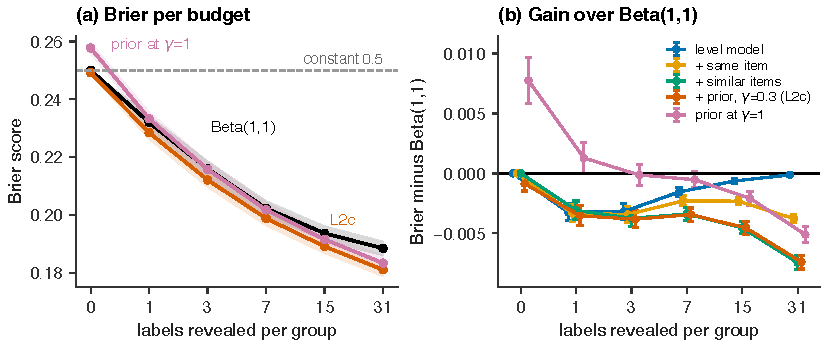
\includegraphics[width=\linewidth]{fig_budget.pdf}
\caption{\textbf{Label sharing carries the gain. The text prior adds little at the chosen weight and hurts at full weight.}
(a)~Brier score per budget for the Beta(1,1) baseline, the narrow model L2c with the text prior at weight $\gamma=0.3$, and L2c at full weight $\gamma=1$.
(b)~Difference from Beta(1,1) as each part is added.
Simulator on the training distribution, \ConfDraws\ fresh draws, 95\% intervals.}
\label{fig:budget}
\end{figure}

\section{Task and official draws}
\label{sec:task}
A subject has eight text fields such as model name, harness and reasoning effort.
An item has its content, metadata and an anonymous benchmark alias.
The function \texttt{predict([subject, item], labeled)} returns a probability and sees every label revealed so far in the draw, for all groups.
With $B_g(k)$ the Brier score of group $g$ after $k$ revealed labels,
\begin{equation}
\mathrm{ALC}_g = 0.1\,B_g(0) + 0.2\,\bigl[B_g(1)+B_g(3)+B_g(7)+B_g(15)\bigr] + 0.1\,B_g(31),
\label{eq:alc}
\end{equation}
and the score of a draw is the mean of $\mathrm{ALC}_g$ over its groups.

All our formative feedback tables share one structure (Appendix~\ref{app:formative}).
A draw holds 8 or 9 groups on the same seven benchmarks, two of which usually contribute two subjects each, and a group is scored on \OffPairsMin\ to \OffPairsMax\ items in almost every case.
The curation guideline states that test subjects are recent systems~\citep{paiec}.

Our reference baseline is the Beta-binomial model with a uniform Beta(1,1) prior, which predicts $(k+1)/(m+2)$ for a group with $k$ correct answers among $m$ revealed labels. The official baseline uses a Beta(2,2) prior and is \PRCOBtwoAbs\% worse in the simulator under test weights (Table~\ref{tab:ladder}).

Three assumptions link our simulator to this setting.
\begin{enumerate}
\item[A1.] Public benchmarks with recent subjects, reweighted to the test pool (Section~\ref{sec:testpool}), stand in for the private ones. If they differ in other ways, simulated gains may not transfer, in either direction.
\item[A2.] Two subjects on one benchmark share most of their items. The feedback cannot confirm this. If it fails, the same-item shift does nothing.
\item[A3.] A revealed label is one recorded response, so we simulate it as a Bernoulli draw with the item's success rate.
\end{enumerate}

\section{Data}
\label{sec:data}
All training data come from measurement-db~\citep{mdb}, which is part of the permitted inventory.
We kept \NBenchKept\ of its benchmarks with binary responses, \TrialRatio\ times more responses than V3 used, and left out four large or single-subject ones (Appendix~\ref{app:data}).
Subject descriptions are sparse.
Only \PctName\% of subject configurations name the model, and \PctRelease\% give a release date.

\section{Method}
\label{sec:method}
\paragraph{Text prior.}
A two-tower network maps the E5 embeddings of the subject text and the item text to a base logit $z_{si}$ for subject $s$ and item $i$.
It is trained with a binomial log loss on all recorded responses, with a free offset per benchmark (Appendix~\ref{app:hyper}).

\paragraph{Label sharing.}
\label{sec:adapt}
Every revealed label with the target's benchmark alias enters the update, whichever subject it belongs to.
On one benchmark, the logit for subject $s$ and item $i$ is
\begin{equation}
\eta_{si} = \gamma z_{si} + c + d_s + u_i, \qquad c\sim\mathcal N(0,\tau_c^2), \quad d_s\sim\mathcal N(0,\tau_d^2).
\label{eq:level}
\end{equation}
Here $\gamma$ scales the text prior, $c$ is a benchmark offset shared by every subject in the draw, $d_s$ is the offset of subject $s$, and $u_i$ is an item shift.
We fit $c$ and all $d_s$ by Newton's method with a Laplace approximation and call this part the \emph{level model}.
A label of another subject moves $c$, and with it every prediction on the benchmark.
The item shift $u_i$ moves item $i$ by the residuals of other subjects on the same item, and by the residuals on items whose E5 embeddings are close to it.
Each shift is one Newton step for an offset shared by the weighted items (Appendix~\ref{app:hyper}).
The prediction averages over the posterior variance of $c+d_s$~\citep{mackay}.

\paragraph{Date and name offsets.}
\label{sec:datename}
L4 adds a fixed subject offset fitted on training groups as a linear function of release date, and L5 also adds an ability per model name.
Both raise predictions for recent strong systems.
The final model does not use them (Section~\ref{sec:res-side}).

\paragraph{Final submission.}
\label{sec:final}
The final model, L3, uses a wide level prior ($\tau_c=2.5$ and $\tau_d=1$, against 1.2 and 0.6 in the narrow models), both item shifts and the text prior at $\gamma=0.3$.
The archive holds E5, the prior network and the code and runs on CPU.
A draw of 8 groups takes \EncDrawMinLo\ to \EncDrawMinHi\ minutes on two virtual CPUs, and no prediction reads a group identifier.
Table~\ref{tab:ladder} lists the other models by the parts they add.

\section{A simulator calibrated to the hidden test pool}
\label{sec:testpool}
We compare models in a simulator of official draws built from public benchmarks.
A draw takes two benchmarks with two subjects each and five with one, as official draws do, and the text prior for each benchmark comes from a network trained without it.
We tuned on development draws and report results on \ConfDraws\ fresh draws per setting (Appendix~\ref{app:sim}).

At first the simulator was far off.
It gave the official baseline, a Beta-binomial model with a Beta(2,2) prior, an ALC of \RSimBtwoACU, while its \OffBetaAllN\ official runs averaged \ROffBetaAllMean.

The official feedback explains the gap.
The baseline predicts one constant $q$ per group, and for a constant the expected calibration error equals $|q-p|$, where $p$ is the group's accuracy.
Before any label the baseline predicts $q=0.5$, so its feedback lists $|p-0.5|$ for every group.
In the baseline runs available when we chose the model, \TpFarShare\% of test groups had accuracy below 20\% or above 80\%, against \ShortTrainFar\% of simulated groups of recent systems.

\emph{Test weights} reweight simulated groups so that their distribution of $|p-0.5|$ matches the test pool.
With them the simulated baseline scores \RSimBtwoACO, and its curve follows the official one at every budget (Figure~\ref{fig:testpool}a).
This match is a weak check on its own, because once the distribution matches, the curve follows mostly from group sizes.
The side of 50\% stays hidden, since flipping every label leaves both scores unchanged.
Section~\ref{sec:res-side} recovers it.

\section{Results}
\label{sec:results}

\subsection{The text prior transfers almost nothing to unseen benchmarks}
\label{sec:res-prior}
In three training variants the best weight of the text prior was the smallest we tried, and ALC improved as the weight shrank (Table~\ref{tab:lobo} in Appendix~\ref{app:extra}).
The best variant beat the label-only baseline by \ShortLoboRel\%.
The prior mainly acts before the first label, and even there it barely helps.
At the chosen weight it lowers the Brier score before any label from 0.250 to \RConfFullBzero, and at full weight it raises it to \RConfGammaOneBzero\ (Figure~\ref{fig:budget}a).
On the platform, the final model's own score before any label is \RSideBzeroLthree, again no better than a constant.
A second encoder, Qwen3-Embedding-0.6B~\citep{qwen3emb}, gave a similarly small gain on a subset, from one set of draws without a standard error, and difficulty ratings from Qwen3-8B~\citep{qwen3} did no better (Appendices~\ref{app:extra} and~\ref{app:judge}).

\subsection{On the training distribution, shared labels carry the gain}
\label{sec:res-structure}
On the training distribution the narrow model lowers ALC by \ShortConfRel\% against the baseline, and \ConfShareStructure\% of this remains without the text prior (Figure~\ref{fig:budget}b).
Each kind of sharing helps at a different budget.
The benchmark offset helps most at 1 to 3 labels, when other subjects on the benchmark add labels that the target lacks.
The same-item shift grows with the budget, and the similar-item shift doubles the gain at 31 labels.

\subsection{On the test pool, a wide prior wins}
\label{sec:res-testpool}
Test weights reorder the models (Table~\ref{tab:ladder}).
On recent subjects without test weights the narrow model L2c is best.
With test weights the wide models lead, and L3 gains \PRCOLthreeAbs\% against \PRCOLtwocAbs\% for L2c. L4 and L5 gain more only while groups keep the training side of 50\%. With \ShortPiGrid\% of groups below 50\%, the smallest share allowed by the official gap between L4 and L3, L3 keeps \PRCSLthreeAbs\% and L5 falls to \PRCSLfiveAbs\% (third column, Section~\ref{sec:res-side}).
Extreme groups need large offsets, and a narrow prior keeps their predictions near the starting value while labels are few.

Two checks show that L3 gains more than a prior that suits extreme groups.
The best Beta prior we tried for this pool, Beta(0.5,0.5), gains only \ShortBhalf\%.
Restricted to the labels of its own group, L3 keeps about half of its gain (\PRCOLthreeownAbs\% against \PRCOLthreeAbs\%).

The text prior adds \ShortTextThree\% at the training side of 50\% and nothing at \ShortPiGrid\% below, where the model without it scores \PRCSWkernel\%.
Under test weights the real V2 and V3 code trails L3 by \ShortRepTwo\% on simulated draws, while without them it matches L3 (Appendix~\ref{app:extra}).

\begin{table}[t]
\centering
\caption{\textbf{Test weights favor wide priors, and once most groups lie below 50\%, the date and name offsets hurt.} Change in ALC against the Beta(1,1) baseline in percent, lower is better. Simulator, subjects released from 2025, 600 fresh draws. The first row gives the baseline ALC. The first two columns keep the training share of groups below 50\% (\ShortTrainBelow\%), and the third sets it to \ShortPiGrid\%, the smallest share allowed by the official gap between L4 and L3 (Section~\ref{sec:res-side}). Standard errors are at most \PRCSSeMax\ points. Appendix~\ref{app:sim} adds all subjects.}
\label{tab:ladder}
\small
\begin{tabular}{lrrr}
\toprule
 & & \multicolumn{2}{c}{Test weights} \\
\cmidrule(lr){3-4}
Model & Training weights & training side & \ShortPiGrid\% below 50\% \\
\midrule
Beta(1,1) baseline, ALC & \PRCUBeta & \PRCOBeta & \PRCSBeta \\
Beta(0.5,0.5) & \PRCUBhalf & \PRCOBhalf & \PRCSBhalf \\
Beta(2,2), the official baseline & \PRCUBtwo & \PRCOBtwo & \PRCSBtwo \\
L1c, narrow level model and same item & \PRCULonec & \PRCOLonec & \PRCSLonec \\
L2c, narrow, all sharing and text prior & \PRCULtwoc & \PRCOLtwoc & \PRCSLtwoc \\
Wide level model & \PRCUWlevel & \PRCOWlevel & \PRCSWlevel \\
\quad + same item & \PRCUWexact & \PRCOWexact & \PRCSWexact \\
\quad + similar items & \PRCUWkernel & \PRCOWkernel & \PRCSWkernel \\
\quad + text prior, $\gamma=0.3$ (L3, final) & \PRCULthree & \PRCOLthree & \PRCSLthree \\
\quad + date offset (L4) & \PRCULfour & \PRCOLfour & \PRCSLfour \\
\quad + name ability (L5) & \PRCULfive & \PRCOLfive & \PRCSLfive \\
L3 with its own group's labels only & \PRCULthreeown & \PRCOLthreeown & \PRCSLthreeown \\
\bottomrule
\end{tabular}
\end{table}

\begin{figure}[t]
\centering
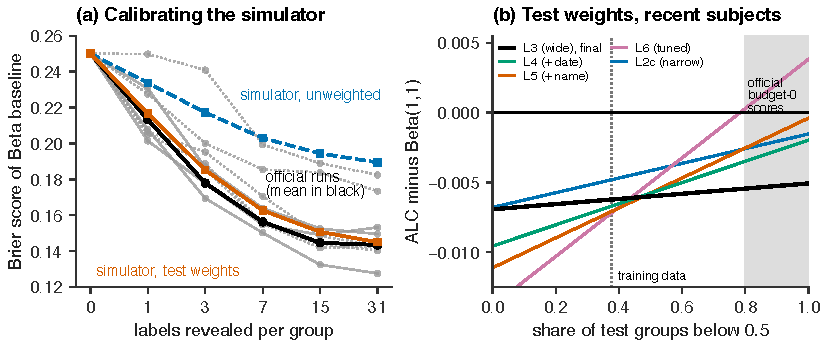
\includegraphics[width=\linewidth]{fig_testpool.pdf}
\caption{\textbf{Test weights reproduce the official baseline curve, and the side of 50\% decides whether date and name offsets help.}
(a)~Brier score per budget of the Beta(2,2) baseline in official runs and in the simulator.
(b)~ALC change against Beta(1,1) under test weights, recent subjects, as the share of groups below 50\% accuracy varies. L6 has larger offsets tuned on development draws (Appendix~\ref{app:sim}).
Dotted line, training share. Shaded, shares allowed by the official gap between L4 and L3 (one-sided 95\% bound).}
\label{fig:testpool}
\end{figure}

\subsection{Official runs point to most test groups lying below 50\%, so the final model drops the offsets}
\label{sec:res-side}
Raising a group's constant prediction from 0.5 to $0.5+s$ changes its Brier score by $s\,(s-2(p-0.5))$, where $p$ is the group's accuracy.
The score rises unless $p>0.5+s/2$.
The date and name offsets raise predictions for recent systems, and the curation guideline says test subjects are recent.

On the platform the offsets raised the Brier score before any label from \RSideBzeroLthree\ for L3 to \RSideBzeroLfour\ for L4 and \RSideBzeroLfive\ for L5. Before any label, every run of L4 and L5 scored worse than every run of L3 (Table~\ref{tab:allruns} in Appendix~\ref{app:formative}).
In training data the offsets help, because \SideTrainAbovePct\% of groups of systems released from 2025 lie above 50\%.

To size the effect we vary the share of simulated groups below 50\% (Figure~\ref{fig:testpool}b).
Even the one-sided 95\% lower bound of the official gap between L4 and L3 needs \ShortPiLow\% of groups below 50\%.
L5 beats L3 only when fewer than \ShortBreakeven\% lie below.
At \ShortPiLow\% and above, L5 loses most of its gain while L3 keeps about 3\%.
We therefore submit L3.
No single share fits all three archives exactly, and Appendix~\ref{app:sim} shows the mismatch.
Official mean ALC cannot settle the choice. L3 averages \ROffLthreeMean, ahead of L5 but behind the mean of all \OffBetaAllN\ baseline runs (\ROffBetaAllMean) and V2 (\ROffVtwoMean), and all these means lie within the spread of one run (Table~\ref{tab:formative}).

\subsection{Single formative runs cannot rank these methods}
\label{sec:res-formative}
The \OffBetaAllN\ official runs of the baseline have a standard deviation of \ROffBetaAllSd\ (Appendix~\ref{app:formative}), and two other teams report similar spreads~\citep{veseluhha,shashwat}.
Each run gets its own draw. Detecting a difference of \QConfFullAbs\ ALC, the size of the label-sharing gain, takes about \RunsNeededOurs\ runs per archive (two-sided 5\% test, 80\% power), against \RunsNeededPaired\ paired draws in the simulator.
The leaderboard keeps each team's best run, which for 20 runs lies about \BestOfTwentyShift\ below the mean, while the final evaluation scores each team once on a common set.

\begin{table}[t]
\centering
\caption{\textbf{Before any label, every L4 and L5 run is worse than every L3 run, while mean ALC does not separate the models.} Official runs, each on its own draw of 8 or 9 groups. $B(0)$ is the mean Brier score before any label. Weight runs set the test weights. L1c and L2c pool builds for the CPU and GPU images. Appendix~\ref{app:formative} lists every run.}
\label{tab:formative}
\small
\begin{tabular}{lrcc}
\toprule
Archive & Runs & ALC, mean (s.e.) & $B(0)$ \\
\midrule
Beta(2,2), weight runs & \OffBetaN & \TabBetaMeanR & 0.250 \\
Beta(2,2), later runs & \OffBetaLaterN & \TabBetaLaterMeanR & 0.250 \\
V2 & \TabVtwoRuns & \TabVtwoMeanR & \TabVtwoBzero \\
V3 & \TabVthreeRuns & \TabVthreeMeanR & \TabVthreeBzero \\
L1c & \TabLonecRuns & \TabLonecMeanR & \TabLonecBzero \\
L2c & \TabLtwoRuns & \TabLtwoMeanR & \TabLtwoBzero \\
L3, final & \TabLthreeRuns & \TabLthreeMeanR & \TabLthreeBzero \\
L4 & \TabLfourRuns & \TabLfourMeanR & \TabLfourBzero \\
L5 & \TabLfiveRuns & \TabLfiveMeanR & \TabLfiveBzero \\
\bottomrule
\end{tabular}
\end{table}

\section{Related work}
\label{sec:related}
Item response theory models success through subject ability and item difficulty~\citep{lord1980,rodriguez2021}, and tinyBenchmarks estimates a benchmark score from a few items with item parameters fitted on that benchmark~\citep{polo2024}, which a cold start lacks.
Observational scaling laws predict scores from capabilities on known benchmarks~\citep{ruan2024}, not item by item on unseen ones.
Text-based difficulty estimation works within a domain~\citep{benedetto2023}, and amortized calibration predicts item difficulty from question content~\citep{truong2025}, the role of our text prior.
Assessors predict a system's success on an instance~\citep{hernandez2022}, and a generic assessor does so for a new model from about 100 reference instances~\citep{pacchiardi2024}. PAIEC gives at most 31 labels, all from the new benchmark.
The level model is a random-intercept logistic model~\citep{efron1975,gelman2007}.

\section{Limitations}
\label{sec:limits}
The test-pool calibration rests on little data, the feedback of three baseline runs and of the L3, L4 and L5 runs in Table~\ref{tab:formative}, all on the same seven benchmarks.
Model selection used it, so our formative runs are not an independent test.
Resampling the bins of the test groups (\BootReps\ replicates) keeps L3 ahead of the baseline in every replicate and ahead of L2c in \BootRCLthreeLtwocP\%, but ignores groups that recur across runs.
The final evaluation draws from the same hidden data~\citep{paiec}, but if it weighs benchmarks differently the gain of L3 may shrink.

Under the less extreme groups of the later baseline runs, L3 loses its lead over L2c (Appendix~\ref{app:sim}).
If the final pool resembled the training data, L2c would beat L3 by about \ShortTwocThreeAllU\%, and if test groups kept the training side of 50\%, L5 would beat L3 by \ShortFiveThreeTrain\%.
The same-item shift relies on assumption A2 but adds only \ShortExactStep\%.
Fresh draws correct for tuning, not for earlier design choices such as the simulator itself.

\section{Conclusion}
\label{sec:conclusion}
In this cold-start task, labels of other systems on the same benchmark were worth more than a frozen-encoder text prior trained on many benchmarks.
Aggregate feedback from a constant baseline told us how extreme the hidden test groups are, and runs of models with shifted predictions pointed to the side of 50\% on which most of them lie. Each finding changed our final model.
Because single runs are this noisy, formative submissions are best compared over repeated runs.

\section*{LLM usage statement}
The author directed the work.
An LLM-based coding assistant was used mainly to write, debug and run code, and it also helped draft and edit the text.
Every result in the tables, figures and text is printed by a script from saved outputs (Appendix~\ref{app:repro}), and the numbers were checked against those outputs before submission.


\begingroup
\small
\begin{thebibliography}{20}
\bibitem[{PAIEC organizers}(2026)]{paiec} Stanford AI Measurement Science. The Predictive AI Evaluation Competition at NeurIPS 2026. Rules, data policy, curation guideline and protocol, 2026. \url{https://aims.stanford.edu/competition}.
\bibitem[{Rogoza}(2026)]{prevreport} Yaroslav Rogoza. Frozen semantic priors with hierarchical evidence adaptation for predictive AI evaluation. Unpublished technical report for PAIEC, 20 October 2026.
\bibitem[{AIMS Foundations}(2026)]{mdb} AIMS Foundations. measurement-db. Hugging Face dataset, revision 54074453, 2026. \url{https://huggingface.co/datasets/aims-foundations/measurement-db}.
\bibitem[{veseluhha}(2026)]{veseluhha} veseluhha. paiec-2026. Public GitHub repository, accessed 4 November 2026. \url{https://github.com/veseluhha/paiec-2026}.
\bibitem[{Srivastav}(2026)]{shashwat} Shashwat Srivastav. s2wish-paiec2026. Public GitHub repository, accessed 4 November 2026. \url{https://github.com/Shashwat-srivastav/s2wish-paiec2026}.
\bibitem[Wang et~al.(2024)]{e5} Liang Wang, Nan Yang, Xiaolong Huang, Linjun Yang, Rangan Majumder, and Furu Wei. Multilingual E5 text embeddings. A technical report. arXiv:2402.05672, 2024.
\bibitem[Zhang et~al.(2025)]{qwen3emb} Yanzhao Zhang, Mingxin Li, Dingkun Long, Xin Zhang, Huan Lin, Baosong Yang, Pengjun Xie, An Yang, Dayiheng Liu, Junyang Lin, Fei Huang, and Jingren Zhou. Qwen3 Embedding. Advancing text embedding and reranking through foundation models. arXiv:2506.05176, 2025.
\bibitem[Yang et~al.(2025)]{qwen3} An Yang and others (Qwen Team). Qwen3 technical report. arXiv:2505.09388, 2025.
\bibitem[Loshchilov and Hutter(2019)]{adamw} Ilya Loshchilov and Frank Hutter. Decoupled weight decay regularization. In \emph{ICLR}, 2019.
\bibitem[MacKay(1992)]{mackay} David J.~C. MacKay. The evidence framework applied to classification networks. \emph{Neural Computation}, 4(5):720-736, 1992.
\bibitem[Lord(1980)]{lord1980} Frederic M. Lord. \emph{Applications of Item Response Theory to Practical Testing Problems}. Lawrence Erlbaum, 1980.
\bibitem[Rodriguez et~al.(2021)]{rodriguez2021} Pedro Rodriguez, Joe Barrow, Alexander Miserlis Hoyle, John P. Lalor, Robin Jia, and Jordan Boyd-Graber. Evaluation examples are not equally informative. How should that change NLP leaderboards? In \emph{ACL}, 2021.
\bibitem[Polo et~al.(2024)]{polo2024} Felipe Maia Polo, Lucas Weber, Leshem Choshen, Yuekai Sun, Gongjun Xu, and Mikhail Yurochkin. tinyBenchmarks. Evaluating LLMs with fewer examples. In \emph{ICML}, 2024.
\bibitem[Ruan et~al.(2024)]{ruan2024} Yangjun Ruan, Chris J. Maddison, and Tatsunori Hashimoto. Observational scaling laws and the predictability of language model performance. In \emph{NeurIPS}, 2024.
\bibitem[Benedetto et~al.(2023)]{benedetto2023} Luca Benedetto, Paolo Cremonesi, Andrew Caines, Paula Buttery, Andrea Cappelli, Andrea Giussani, and Roberto Turrin. A survey on recent approaches to question difficulty estimation from text. \emph{ACM Computing Surveys}, 55(9), 2023.
\bibitem[Efron and Morris(1975)]{efron1975} Bradley Efron and Carl Morris. Data analysis using Stein's estimator and its generalizations. \emph{Journal of the American Statistical Association}, 70(350):311-319, 1975.
\bibitem[Gelman and Hill(2007)]{gelman2007} Andrew Gelman and Jennifer Hill. \emph{Data Analysis Using Regression and Multilevel/Hierarchical Models}. Cambridge University Press, 2007.
\bibitem[Truong et~al.(2025)]{truong2025} Sang Truong, Yuheng Tu, Percy Liang, Bo Li, and Sanmi Koyejo. Reliable and efficient amortized model-based evaluation. In \emph{ICML}, 2025.
\bibitem[Hern{\'a}ndez-Orallo et~al.(2022)]{hernandez2022} Jos{\'e} Hern{\'a}ndez-Orallo, Wout Schellaert, and Fernando Mart{\'i}nez-Plumed. Training on the test set. Mapping the system-problem space in AI. In \emph{AAAI}, 2022.
\bibitem[Pacchiardi et~al.(2024)]{pacchiardi2024} Lorenzo Pacchiardi, Lucy G. Cheke, and Jos{\'e} Hern{\'a}ndez-Orallo. 100 instances is all you need. Predicting the success of a new LLM on unseen data by testing on a few instances. arXiv:2409.03563, 2024.
\bibitem[Zheng et~al.(2023)]{zheng2023} Lianmin Zheng, Wei-Lin Chiang, Ying Sheng, Siyuan Zhuang, Zhanghao Wu, Yonghao Zhuang, Zi Lin, Zhuohan Li, Dacheng Li, Eric P. Xing, Hao Zhang, Joseph E. Gonzalez, and Ion Stoica. Judging LLM-as-a-judge with MT-Bench and Chatbot Arena. In \emph{NeurIPS Datasets and Benchmarks}, 2023.
\end{thebibliography}
\endgroup

\appendix
\section{Reproduction}
\label{app:repro}
Paths are relative to the root of the code repository \url{https://github.com/123yaroslav/paiec2026}, which also holds the sources and data of this report. All CPU steps, the simulator and the runtime tests ran on the Mac with Python 3.12.12, torch 2.14.1, transformers 5.19.0, numpy 2.5.3, pandas 3.0.6, pyarrow 25.0.1 and huggingface\_hub 1.33.0. GPU steps ran on Google Colab L4 runtimes with their preinstalled torch and transformers, driven by the colab command-line tool 0.7.4. Two mismatches remain between training and runtime. The prior's training weights give groups with repeated trials less weight than the score does, and training embeddings were stored in float16 while the runtime uses float32. The corpus omits \NBenchNotFetched\ large or single-subject benchmarks and keeps the most-answered items of large benchmarks (Appendix~\ref{app:data}). Because in-memory caches last one budget, L3 and L5 encode \EncPerBudgetLo\ to \EncPerBudgetHi\ texts per budget of a draw. On a two-vCPU Colab CPU runtime with one torch thread this costs \EncTextSec\ seconds per text and \EncLoadSec\ seconds per model load, so a run reaches the 8-hour limit only at about \EncMaxGroups\ groups, against 8 or 9 in a formative run.

\paragraph{1. Download and build the corpus (local CPU).} The download fetches benchmark tables at the pinned revision and skips the four benchmarks listed in Appendix~\ref{app:data}.
\begin{lstlisting}
python - <<'EOF'
import json
from huggingface_hub import snapshot_download
R, REV = "aims-foundations/measurement-db", "54074453da7b9911be0f48e4c560be547bc84d21"
skip = {"mind2web", "naturalreasoning", "swe_smith", "tensortrust"}
keep = [b for b in json.load(open("colab_jobs/binary_benchmarks.json")) if b not in skip]
snapshot_download(R, repo_type="dataset", revision=REV, local_dir="data/mdb_full",
    allow_patterns=["*/formatted_tables/benchmarks.parquet", "*/formatted_tables/subjects.parquet"]
    + [f"{b}/formatted_tables/{t}.parquet" for b in keep for t in ("responses", "items")])
EOF
RAW=data/mdb_full OUT=data/corpus_full RUNTIME_DIR=v5 EMBED=0 SKIP_FETCH=1 python colab_jobs/build_corpus.py
\end{lstlisting}

\paragraph{2. Embeddings, priors and held-out logits (one L4 GPU).} We run jobs on Colab through \texttt{colab\_jobs/ctl.py} (budget check, upload, watch, download with SHA-256 check, stop) and \texttt{colab\_jobs/supervisor.py} (status file, stall kill, release of idle machines). On the GPU machine, \texttt{/content/run} holds \texttt{v5/\{spec,encoder,textproj,adapt\}.py} and the job scripts, and \texttt{/content/work} holds the corpus.
\begin{lstlisting}
python /content/run/embed_texts.py
python /content/run/train_eval.py cv --tag A
python /content/run/train_eval.py cv --tag B --bench-offset 1
python /content/run/train_eval.py cv --tag C --bench-offset 1 --dropout 0.3 --wd 0.01 --epochs 2
cd /content/run4 && RUNTIME_DIR=/content/run python export_z.py --tag B   # needs train_eval3.py in /content/run3
\end{lstlisting}
The last command writes \texttt{pairs\_z.parquet} with held-out logits from five benchmark folds and \texttt{prior\_B.npz}, the prior trained on all benchmarks (SHA-256 \texttt{486b104f\ldots}). The encoder comparison runs \texttt{feat\_bakeoff.py} and \texttt{train\_eval2.py} with \texttt{--item-keys-file} on the 600-item subset. The subject offsets come from \texttt{python colab\_jobs/fit\_subject\_priors.py}, which writes \texttt{date\_prior.json}, \texttt{v5/name\_ability.json} and \texttt{name\_ability\_folds.json} and reproduces our files exactly.

\paragraph{3. Test-pool statistics and simulations (local CPU).} The first command computes the statistics of Section~\ref{sec:testpool} and Appendix~\ref{app:sim}. The others reproduce Tables~\ref{tab:ladder} and~\ref{tab:ladderfull}, Figure~\ref{fig:budget}, Figure~\ref{fig:testpool}b and Section~\ref{sec:res-side}, the runtime replays and the encoder cost. The baseline script reuses the ladder's draws, and \texttt{make\_numbers.py} stops if they differ.
\begin{lstlisting}
cd reports/paiec_v5_report
python -B scripts/test_pool_stats.py
python -B scripts/sim_ladder.py --tag recent_conf --min-date 2025-01-01 --seed0 300000  # also all_conf, and dev tags with --seed0 0
python -B scripts/sim_baselines.py --tag recent_conf --min-date 2025-01-01 --seed0 300000  # also all_conf
python -B scripts/sim_baselines.py --tag recent_conf --min-date 2025-01-01 --seed0 300000 --only beta,L3,L3_own \
  --out baselines_l3                                                                       # also all_conf
python -B scripts/side_of_half.py                                                        # side of 50%
python -B scripts/sim_confirm.py --draws 600 --seed0 100000                              # Figure 1
python -B scripts/extra_stats.py                                                         # judge, name ability, replays
cd ../.. && EX=bertaqa,cellverse,cruxeval,engdesign,erbench,kernelbench,liveaopsbench,researchcodebench,tau2_bench
python -B colab_jobs/replay_runtime.py UNZIPPED_V2_DIR colab_jobs/results/replay_v2.parquet --seeds 0:120 \
  --min-date 2025-01-01 --exclude $EX
python -B reports/paiec_v5_report/scripts/record_encoder_texts.py UNZIPPED_L5_DIR texts.json
python reports/paiec_v5_report/scripts/time_encoder.py texts.json encode_timing.json  # CPU machine, next to v5/encoder.py
\end{lstlisting}
The last two commands give the encoder cost of Section~\ref{sec:final}. The first writes item texts from measurement-db, so its output is not in the repository.
The ladder and confirmation scripts import frozen copies of the simulator (\texttt{scripts/sim\_official\_v2\_snapshot.py}, SHA-256 \texttt{8da09880\ldots}, and \texttt{scripts/sim\_official\_snapshot.py}). The paired simulator rows came from \texttt{sim\_official.py --emb data/corpus\_full/item\_emb.npy --draws 120 --min-date 2025-01-01 --exclude \$EX --dump colab\_jobs/results/sim\_dump\_recent\_ex.parquet} with the variants Beta, L1c, L3, L4 and L5. The dump stores raw per-group ALC and $p$, so test weights are applied afterwards.

\paragraph{4. Final archive.} The first command rebuilds L3 and the last checks it with the validator of the organizers' starting kit, which is not part of our repository. The second builds L5.
\begin{lstlisting}
P=colab_jobs/results/exportB/work/results
python v5/build_zip.py $P/prior_B.npz $P/prior_B.json 2.5 1.0 0.3 dist/v5/L3_wide_prior.zip \
  '{"use_prior": true, "item_exact": 1.0, "item_kernel": [0.03, 3.0]}'
python v5/build_zip.py $P/prior_B.npz $P/prior_B.json 2.5 1.0 0.3 dist/v5/L5_wide_date_name.zip \
  '{"use_prior": true, "item_exact": 1.0, "item_kernel": [0.03, 3.0], "name_scale": 0.8, "date_prior": '"$(cat colab_jobs/results/date_prior.json)"'}'
python starting_kit/tools/check_submission_zip.py dist/v5/L3_wide_prior.zip
\end{lstlisting}
Our L3 archive (Codabench submission 1033014) has SHA-256
\begin{center}\texttt{a47150effc0761d29b206ccb548d3c7da6a063e7a22072a352e60dc5b15f7ee7}.\end{center}
We built it before the offset code entered \texttt{model.py}. A rebuild adds that code and the unused name table, and on 360 synthetic calls with 0, 5 and 30 labels it returns identical predictions. The L5 archive has SHA-256 \texttt{2d8b7034\ldots}.
 The script \texttt{build\_zip.py} takes the five E5 files from the V3 archive or, if it is absent, from the hub at the pinned revision, and checks their SHA-256. A rebuild gives identical file contents.

\paragraph{5. Formative runs and this report.} The first three commands resubmit an uploaded archive, collect the scores of finished runs and record the runs still waiting in the queue. The others rebuild the numbers, the figures and this PDF.
\begin{lstlisting}
python scripts/resubmit.py L5_wide_date_name.zip 3 --label L5
python scripts/track.py
python scripts/queue_snapshot.py
cd reports/paiec_v5_report && python -B scripts/make_numbers.py && python -B scripts/make_figures.py
pdflatex main.tex && pdflatex main.tex
\end{lstlisting}

\section{Training corpus}
\label{app:data}
All training data come from measurement-db at revision \texttt{54074453}~\citep{mdb}.
Of its \NBenchAll\ benchmarks, \NBenchBinary\ have binary responses.
We did not download \NBenchNotFetched\ of them (\SkippedFetch), which have one to three subjects each and include two with more than 500,000 items, and \NBenchNoBinary\ more had no binary rows.
Each of the remaining \NBenchKept\ benchmarks keeps at most 4,000 items, the ones answered by the most subjects, and we store the number of recorded trials $n$ and successes $k$ of every subject-item pair.
A subject is the exact tuple of its eight fields, so one base model under another harness is a different subject.
Of the \NSubjectConfigs\ subject configurations, \PctName\% have a model name, \PctRelease\% a release date and \PctEffort\% a reasoning effort.

\begin{table}[ht]
\centering
\caption{\textbf{\VF\ trains on about \TrialRatio\ times more recorded responses than V3.} Groups are subject-benchmark pairs. Accuracies are benchmark-weighted means over groups with at least 80 items.}
\label{tab:corpus}
\small
\begin{tabular}{lrr}
\toprule
 & V3 training data & \VF\ corpus \\
\midrule
Benchmarks & 5 & \NBenchKept \\
Recorded binary responses & \VthreeResponses & \NTrials \\
Subject-item pairs and items & & \NPairs\ and \NItems \\
Subject configurations (with responses) & & \NSubjectConfigs\ (\NSubjectsWithPairs) \\
Groups with at least 80 items & \VthreeGroups\ (all sizes) & \NGroupsEighty\ on \NBenchGroupsEighty\ benchmarks \\
Mean group accuracy, all subjects & & \TrainP\ (\TrainAbove\% above 0.5) \\
Mean group accuracy, released from July 2025 & & \RecentP\ (\RecentAbove\% above 0.5) \\
\bottomrule
\end{tabular}
\end{table}

\section{Model details and hyperparameters}
\label{app:hyper}
\paragraph{Prior network.} Items and subjects are embedded with the frozen \texttt{intfloat/multilingual-e5-small} encoder~\citep{e5} at revision \texttt{614241f}, with the recipe of V3. An item text is its metadata line followed by its task, and a subject text lists its fields. Two towers, each a two-layer perceptron with 256 Gaussian error linear units, map the subject input (E5 vector and release date) and the item input (E5 vector and text length) to $h_s$ and $h_i$. The logit is $z_{si} = a(h_s) + b(h_i) + \langle U h_s, V h_i\rangle/\sqrt{32}$ with linear heads $a$, $b$ and rank-32 projections $U$, $V$. Training minimizes the binomial log loss of the counts $(n,k)$ of every pair, with weight $1/(nT_g)$ for a pair in group $g$ with $T_g$ trials. Each benchmark gets a free offset during training, and the mean offset is folded into the intercept afterwards.

\paragraph{Item shift.} The item shift uses residuals of the labeled pairs under the level model. For labeled pair $j$ with subject $s_j$ and item $i_j$, let $\hat p_j=\sigma(\gamma z_j + o_{s_j} + m_{s_j})$, $r_j = y_j-\hat p_j$ and $w_j=\hat p_j(1-\hat p_j)$, where $m_s$ is the posterior mean of $c+d_s$, $o_s$ the fixed subject offset of L4 and L5 (zero in L3) and $y_j$ the label. For a kernel $K$ with prior variance $\sigma_K^2$,
\begin{equation}
u_i = \sum_{K} \frac{\sigma_K^2 \sum_j K(i,i_j)\, r_j}{1+\sigma_K^2\sum_j K(i,i_j)\, w_j},
\label{eq:shift}
\end{equation}
which is one Newton step from zero for an offset shared by the target item and the labeled items, weighted by $K$.
The same-item kernel $K(i,i')=\mathbf 1[i=i']$ has variance $\sigma_e^2$. The similar-item kernel $K(i,i')=\exp\bigl((\cos(e_i,e_{i'})-1)/h\bigr)$ on E5 vectors has bandwidth $h$ and variance $\sigma_k^2$.
With $\eta^*_{si}=\gamma z_{si}+o_s+m_s+u_i$ and $v_s$ the posterior variance of $c+d_s$, the prediction is $p_{si}=\sigma\bigl(\eta^*_{si}/\sqrt{1+\pi v_s/8}\bigr)$~\citep{mackay}.
L3 uses $\sigma_e^2=1$, $h=0.03$ and $\sigma_k^2=3$. The narrow models use $\tau_c=1.2$, $\tau_d=0.6$ and $\sigma_e^2=2$.

\paragraph{Date and name offsets.} The fixed offset $o_s$ adds two subject priors fitted on training groups with at least 80 items. The date prior is $\DateA + \DateB\,t$, with $t$ the years from 2023-01-01 to the release date clipped to $[-3,4]$, and $\DateAzero$ for an unknown date, fitted by benchmark-weighted least squares to group logit accuracy. The name ability of a normalized model name is the mean, over its training groups, of the group logit minus the benchmark's mean logit, shrunk with a pseudo-count of 2 and clipped to $\pm2.5$. It enters with weight 0.8, and the submission holds \NameCount\ names. In simulation the name ability comes from the four other benchmark folds only. There it has a positive within-benchmark Spearman correlation with group accuracy on \NamePos\% of \NameBench\ held-out benchmarks with at least five named groups (median \NameMedian).

\paragraph{Final archive.} L3 holds the E5 weights, the prior network and the code (\ArchiveFinalMB\ megabytes) and declares no \texttt{models.txt}. It runs on CPU with one prediction worker, which the platform restarts at every budget, so the encoder runs again for each budget. Caches of embeddings, logits and level fits are keyed by content hashes, so no prediction depends on earlier calls.

\paragraph{Text projection.} Each text gets the E5 query prefix, and hidden states are mean-pooled under the attention mask and normalized to unit length. Texts longer than 8,192 characters keep a head, a middle and a tail span. After tokenization, inputs longer than 510 tokens keep four spans of 128, 127, 127 and 128 tokens spread evenly over the text. A JSON chat transcript that ends in a user turn keeps up to 512 characters of system messages and the final user message. The item text is the first 300 characters of the item features followed by this projection. The subject text lists name, provider, release date, harness with version, reasoning effort and the first 300 characters of the extras.
\paragraph{Prior training.} Subject input is the E5 vector, the years from 2023 to the release date clipped to $\pm5$ and a missing-date flag. Item input is the E5 vector and $\log(1+\text{characters})/10$. Hidden width 256, rank 32, dropout 0.1, AdamW~\citep{adamw} with learning rate $2\times10^{-3}$ and weight decay $10^{-4}$, one-cycle schedule with 10\% warm-up, batch 8,192, 4 epochs, seed 99 for the final prior and the fold index for fold priors.
\paragraph{Leave-benchmark-out grid.} The grid crosses $\tau_c\in\{0.8,1.2,1.8,2.5,3.5\}$ with $\tau_d\in\{0.5,0.8,1.2\}$ and $\gamma\in\{0.3,0.45,0.6,0.75,0.9\}$, 75 configurations in total. The first run used $\gamma$ from \LoboInitGammaMin\ upward and was \LoboInitRelAbs\% worse than \BB.
\paragraph{Simulator grids.} Newton iterations stop after 25 steps or when the largest step is below $10^{-7}$. All three grids of the official-structure simulator used \GridDraws\ development draws and include the Beta(1,1) baseline. Here $\gamma=0$ means no text prior.
Grid 1 (no test weights, all subjects, \GridN\ configurations) crossed $\tau_c\in\{0.9,1.2,1.6\}$, $\tau_d\in\{0.6,0.8,1.1\}$, $\sigma_e^2\in\{2,4,8\}$, $h\in\{0.02,0.03,0.05\}$, $\sigma_k^2\in\{1,1.5,3\}$ and $\gamma\in\{0,0.3\}$. Its best difference was \GridDiff\ (standard error \GridSe), and it chose the narrow configuration.
Grid 2 (earlier test-weight shares, all subjects, 289 configurations) crossed $\tau_c\in\{2,2.5,3.5,5\}$, $\tau_d\in\{0.8,1,1.4,2\}$, $\sigma_e^2\in\{1,2,4\}$, $\sigma_k^2\in\{1.5,3,6\}$ at $h=0.03$, and $\gamma\in\{0,0.3\}$. It chose the wide level prior of L3.
Grid 3 (earlier test-weight shares, subjects from 2025, 326 configurations with L5) crossed $\tau_c\in\{2,2.5,3.2\}$, $\tau_d\in\{0.8,1,1.3\}$, $\sigma_e^2\in\{0.5,1,2\}$, $\gamma\in\{0.2,0.3,0.45\}$, name weight $\{0.8,1.2\}$ and date weight $\{1,1.5\}$ at $\sigma_k^2=3$ and $h=0.03$. Its best configuration is L6.
Top lines are in \texttt{colab\_jobs/results/sim\_testw\_grid2.log} and \texttt{sim\_grid3\_recent.log}.
Of the 600 draws of the unweighted confirmation run, \ConfNine\ hold 9 groups, \ConfEight\ hold 8 and \ConfSeven\ hold 7.
\paragraph{Judge prompt.} The system message reads ``You estimate how hard a task is for current frontier AI systems. Read the task and rate its difficulty on a scale from 1 to 9, where 1 means almost every AI system solves it correctly and 9 means almost none does. Answer with a single digit only.'' The user message is ``Task:'' followed by the item text, truncated to 1,024 tokens of head and tail, and ``Difficulty (1-9):''. Thinking mode is off.

\section{Simulator, test weights and the side of 50\%}
\label{app:sim}
\paragraph{Baseline.} The \BB\ baseline predicts $(k+a)/(m+2a)$ for every evaluation item of a group with $m$ revealed labels and $k$ successes. Simulations use $a=1$ and the official archive uses $a=2$, which is worse by \ConfBetaTwoAbs\ ALC in simulation (standard error \ConfBetaTwoSe).

\paragraph{Leave-benchmark-out simulation.} We split the \NBenchKept\ benchmarks into \LoboFolds\ random folds, train the prior on four and simulate on groups of the fifth with at least 80 items, subsampled to 80 to 160 items. Draws of the level model collect groups up to 1,000 items, 60 per fold, from \LoboGroups\ held-out groups.

\paragraph{Official-structure simulator.} A draw picks 2 benchmarks whose two sampled subjects share 88 to 152 items and 5 benchmarks with one subject, and drops groups beyond 1,000 items, so most draws hold 8 groups. Each group is split in half independently. Base logits come from the prior trained without the pair's benchmark fold. Options restrict subjects to those released from 2025 (\LadRDBench\ benchmarks) and apply test weights. Seeds 0 to 599 serve development, the tuning grids used \GridDraws\ of them, and 600 seeds from 100,000, 200,000 and 300,000 serve one confirmation run each. Standard errors treat the draw as the unit.

\paragraph{Runtime replays and formative runs.} We ran the real V2 and V3 submission code on the simulator's draws (recent subjects, seeds from 0) and paired each group with the simulator's L3, L5 and \BB\ rows. These draws exclude the nine benchmarks that V2 or V3 trained or tuned on. On the platform each submission is scored on a new random draw, so we resubmit an archive several times and report the mean and standard error across runs.

\paragraph{Test weights.} For a group whose prediction is one constant $q$, the Brier score is $p(1-p)+(q-p)^2$ and the expected calibration error is $|q-p|$. The official baseline therefore gives $|p-0.5|$ at budget 0 for every group, and $p(1-p)=B_{31}-\mathrm{ECE}_{31}^2$ agrees with it to $10^{-6}$. The shares of $|p-0.5|$ in the bins $[0,0.1)$, $[0.1,0.2)$, $[0.2,0.3)$, $[0.3,0.4)$ and $[0.4,0.5]$ are \TpShareOwn. The tuning grids used an earlier estimate (\TpShareSim) that placed one group in a different bin, and all confirmation runs use the shares above. With test weights the simulated Beta(2,2) baseline scores \SimBtwoACO\ on all subjects and \SimBtwoRCO\ on recent subjects, against \SimBtwoACU\ and \SimBtwoRCU\ without them. The three weight runs average \OffBetaMean\ (standard error \OffBetaSe). Later runs, made after the model choice, scored \OffBetaLaterRuns, and all \OffBetaAllN\ runs average \OffBetaAllMean\ (standard error \OffBetaAllSe). Under the shares of the \TpLaterGroups\ less extreme evaluations of the later runs, the gaps of L3 to Beta(1,1) and to L2c are \ShLaterRCLthreeBeta\ and \ShLaterRCLthreeLtwoc. Official runs of V2 (mean \OffVtwoMean, \OffVtwoN\ runs) and V3 (\OffVthreeMean, \OffVthreeN) lie within one standard error of the Beta(2,2) mean. Only such aggregate statistics and per-archive scores enter model selection.

\paragraph{Absolute results.} Table~\ref{tab:ladderfull} gives the first two columns of Table~\ref{tab:ladder} as absolute ALC differences and adds all subjects and some variants. In the wide level model, sharing only the benchmark offset is worth \PairRCLevelShareOAbs\ (standard error \PairRCLevelShareOSe) under test weights on recent subjects and needs no shared items, and the same-item step adds \PairRCExactStepOAbs.

\begin{table}[ht]
\centering
\caption{\textbf{Simulator results in absolute ALC.} Official-structure simulator, the same 600 confirmation draws (seeds from 300,000) in each population. The first row is the Beta(1,1) ALC, other rows are differences from it, lower is better. Standard errors are 0.0001 to 0.0003 per cell.}
\label{tab:ladderfull}
\small
\begin{tabular}{lrrrr}
\toprule
Subjects & all & all & recent & recent \\
Test weights & no & yes & no & yes \\
\midrule
\BB\ ALC & \LadACUBeta & \LadACOBeta & \LadRCUBeta & \LadRCOBeta \\
\BB, Beta(0.5,0.5) & \LadACUBhalf & \LadACOBhalf & \LadRCUBhalf & \LadRCOBhalf \\
\BB, Beta(2,2), official prior & \LadACUBtwo & \LadACOBtwo & \LadRCUBtwo & \LadRCOBtwo \\
L1c, narrow level + same item & \LadACULonec & \LadACOLonec & \LadRCULonec & \LadRCOLonec \\
L2c, narrow, all sharing + E5 prior & \LadACULtwoc & \LadACOLtwoc & \LadRCULtwoc & \LadRCOLtwoc \\
Wide level model & \LadACUWlevel & \LadACOWlevel & \LadRCUWlevel & \LadRCOWlevel \\
\quad + same item & \LadACUWexact & \LadACOWexact & \LadRCUWexact & \LadRCOWexact \\
\quad + similar items & \LadACUWkernel & \LadACOWkernel & \LadRCUWkernel & \LadRCOWkernel \\
\quad + E5 prior, $\gamma=0.3$ (L3, final) & \LadACULthree & \LadACOLthree & \LadRCULthree & \LadRCOLthree \\
\quad + date prior (L4) & \LadACULfour & \LadACOLfour & \LadRCULfour & \LadRCOLfour \\
\quad + name ability (L5) & \LadACULfive & \LadACOLfive & \LadRCULfive & \LadRCOLfive \\
L5 without the E5 prior & \LadACULfivent & \LadACOLfivent & \LadRCULfivent & \LadRCOLfivent \\
Wide level model, own labels only & \LadACUWown & \LadACOWown & \LadRCUWown & \LadRCOWown \\
L3, own labels only & \LadACULthreeown & \LadACOLthreeown & \LadRCULthreeown & \LadRCOLthreeown \\
L6, best of a grid on recent dev draws & \LadACULsix & \LadACOLsix & \LadRCULsix & \LadRCOLsix \\
\bottomrule
\end{tabular}
\end{table}

\paragraph{Side of 50\%.} On the platform the budget-0 Brier score was \SideBzeroLthree\ for L3 (standard error \SideBzeroLthreeSe, \SideBzeroLthreeGroups\ group evaluations), \SideBzeroLfour\ for L4 (\SideBzeroLfourSe) and \SideBzeroLfive\ for L5 (\SideBzeroLfiveSe). We reweight simulated groups within each $|p-0.5|$ bin so that a share $\pi$ lies below 0.5. At the training share of \SideTrainShare\ the simulated budget-0 gap between L4 and L3 is \SideGapLfourSimTrain, and even at $\pi=1$ it reaches only \SideGapLfourSimMax, below the official \SideGapLfour\ (standard error \SideGapLfourSe). The one-sided lower 95\% bound of the official gap needs $\pi\ge\SidePiLow$ (two-sided, \SidePiLowTwo). No single share fits all three archives. The official L4 and L5 scores alone \SidePiFromPhrase, and the L4 score alone needs $\pi\ge\SidePiFromLfourLow$, but the simulated L3 rises to \SideLthreeSimAtLow\ at $\pi=\SidePiLow$ against its official \SideBzeroLthree, which alone points to \SidePiFromLthree. The gap between L4 and L3 removes the part they share, the text prior, so we use it. L5 beats L3 only for $\pi<\SideBreakeven$. L3 is better by \SideFiveThreeLowAbs\ at $\pi=\SidePiLow$ and by \SideFiveThreeOneAbs\ at $\pi=1$ (standard errors about 0.0001), and the tuned L6, with larger offsets, falls behind \BB\ for $\pi>\SideLsixCross$. The difference of L3 from Beta(1,1) stays between \SideThreeLo\ and \SideThreeHi\ over the whole range. On all subjects L5 and L3 differ by at most \SideAllLoAbs, because older subjects get small offsets. Figure~\ref{fig:testpool}b has standard errors of at most \SidePlotSe.

\section{Leave-benchmark-out results and runtime replays}
\label{app:extra}
\begin{table}[t]
\centering
\caption{\textbf{In every variant the best prior weight is the smallest one tried.} Leave-benchmark-out ALC with the level model, best $(\tau_c,\tau_d)$ per row, lower is better. Each block has its own draws and baseline. Variant C adds dropout 0.3, weight decay 0.01 and 2 epochs to B.}
\label{tab:lobo}
\small
\begin{tabular}{llrr}
\toprule
Data & Prior & ALC & vs \BB \\
\midrule
Full corpus & \BB, Beta(1,1) & \LoboBeta & \\
 & B, $\gamma=0.3$ & \LoboBGammaThree & \LoboBRel\% \\
 & B, $\gamma$ from 0.45 to 0.9 & \LoboBGammaFourFive\ to \LoboBGammaNine & \\
 & A (no benchmark offsets), $\gamma=0.3$ & \LoboA & \LoboARel\% \\
 & C (more regularization), $\gamma=0.3$ & \LoboC & \LoboCRel\% \\
\midrule
600-item subset & \BB, Beta(1,1) & \BakeBeta & \\
 & E5 prior, $\gamma=0.3$ & \BakeEfive & \BakeEfiveRel\% \\
 & Qwen3-Embedding-0.6B prior, $\gamma=0.3$ & \BakeQwen & \BakeQwenRel\% \\
\bottomrule
\end{tabular}
\end{table}

With test weights, L3 beat the real V2 code by \RepTwoTDiffThreeAbs\ (standard error \RepTwoTDiffThreeSe, \RepTwoDraws\ draws, \RepTwoGroups\ groups) and V3 by \RepThreeTDiffThreeAbs\ (\RepThreeTDiffThreeSe, \RepThreeDraws\ draws). Without weights the differences were \RepTwoUDiffThree\ (\RepTwoUDiffThreeSe) and \RepThreeUDiffThree\ (\RepThreeUDiffThreeSe).
V2 was close to \BB\ under test weights (\RepTwoTVsBeta, standard error \RepTwoTVsBetaSe) and better without them (\RepTwoUVsBeta).
So V2 and V3 match L3 on the training distribution but fall behind it on the extreme test pool, where their narrow priors lose the gain over \BB.
A replay of the L5 runtime on \RepCheckDraws\ draws (\RepCheckGroups\ groups) matched the simulator within \RepCheckDiff\ ALC per group on average, and a rebuild of L3 with that code returns identical predictions (Appendix~\ref{app:repro}).


\section{The LLM difficulty judge}
\label{app:judge}
Following the use of LLMs as graders~\citep{zheng2023}, Qwen3-8B~\citep{qwen3} rated item difficulty from 1 to 9 as the expected digit of its next-token distribution, with the prompt of Appendix~\ref{app:hyper}.
It rated \JudgeRated\ of \JudgeItems\ sampled items before we stopped the run to save compute, so long items are missing.
The within-benchmark Spearman correlation between rating and item accuracy had median \JudgeMedian\ and was negative, the useful direction, on \JudgeNeg\% of \JudgeBench\ benchmarks. Between benchmarks it was \JudgeBetween.
In the simulator on rated items with test weights, the best weight of \JudgeSimWeight\ on the standardized rating improved ALC by only \JudgeSimGain\ and hurt budget 0.

\section{Formative runs}
\label{app:formative}
Table~\ref{tab:allruns} lists every finished formative run of our team. V1 and the V3 variant with an uncertainty band are earlier entries not described here.
\begin{table}[ht]
\centering
\caption{\textbf{All finished formative runs.} Means over groups of one draw each. $B_0$ and $B_{31}$ are mean Brier scores at budgets 0 and 31.}
\label{tab:allruns}
\small
\begin{tabular}{rlrrrrr}
\toprule
Submission & Archive & Groups & Benchmarks & ALC & $B_0$ & $B_{31}$ \\
\midrule
\OfficialRows
\bottomrule
\end{tabular}
\end{table}

\section{Training sources, pretrained models and compute}
\label{app:disclosure}
\paragraph{Training sources.} All training and development data come from measurement-db at revision \texttt{54074453da7b9911be0f48e4c560be547bc84d21}, restricted to the \NBenchKept\ binary benchmarks of Section~\ref{sec:data}. No other data source was used for training, tuning or simulation. The test weights use aggregate statistics of our own formative feedback (Section~\ref{sec:testpool}). Earlier entries V2 and V3 used four and five benchmarks of the same inventory~\citep{prevreport}.
\paragraph{Pretrained models.} No model was fine-tuned, and no paid API was used. Table~\ref{tab:models} lists every pretrained model we ran.
\begin{table}[ht]
\centering
\caption{\textbf{Pretrained models used in this work.} Only E5 runs inside the submission.}
\label{tab:models}
\footnotesize
\begin{tabular}{l>{\scriptsize\ttfamily}l>{\raggedright\arraybackslash}p{2.7cm}}
\toprule
Model & \normalfont\footnotesize Revision & Use \\
\midrule
\texttt{intfloat/multilingual-e5-small} & 614241f622f53c4eeff9890bdc4f31cfecc418b3 & frozen encoder in training and in the submission \\
\texttt{Qwen/Qwen3-Embedding-0.6B} & 97b0c614be4d77ee51c0cef4e5f07c00f9eb65b3 & encoder comparison only \\
\texttt{Qwen/Qwen3-4B} & 1cfa9a7208912126459214e8b04321603b3df60c & feature extraction, stopped before it finished \\
\texttt{Qwen/Qwen3-8B} & b968826d9c46dd6066d109eabc6255188de91218 & difficulty judge \\
\bottomrule
\end{tabular}
\end{table}
\paragraph{Compute.} GPU work ran on Google Colab L4 instances, and one Colab CPU runtime timed the encoder. Together they used \ColabUnits\ compute units of our own. Corpus building, simulation, replays, packaging and this report ran on an Apple M4 laptop.

\end{document}
